\documentclass[nonacm, sigconf]{acmart}
% \documentclass[sigconf,screen,balance]{acmart}
\settopmatter{printacmref=false} % Removes citation information below abstract
\renewcommand\footnotetextcopyrightpermission[1]{} % removes footnote with conference information in first column
\pagestyle{plain} % removes running headers

\usepackage{hyperref}
\usepackage[hyphenbreaks]{breakurl}
\usepackage{balance}
\usepackage{url}
\usepackage{color}
\usepackage{caption}
\usepackage{diagbox}
\usepackage{subfigure}
\usepackage{multirow}
\usepackage{booktabs}
\usepackage{epsfig,endnotes}
\usepackage{enumitem}
\newcommand{\RNum}[1]{\uppercase\expandafter{\romannumeral #1\relax}}

\newcommand{\model}{{\mathcal{F}_{\theta}}}
\newcommand{\orgmodel}{{\mathcal{F}_{o}}}
\DeclareMathOperator{\sign}{sign}


\DeclareMathOperator*{\argmin}{argmin}

\newcommand{\para}[1]{{\vspace{2pt} \noindent \textbf{#1}
    \hspace{6pt}}}

% \newcommand{\subpara}[1]{{\vspace{1.0pt} \noindent \emph{#1}
%     \hspace{6pt}}}

\newcommand{\subpara}[1]{{\vspace{1.0pt} \textbf{#1}
    \hspace{4pt}}}

\newcommand{\fixme}[1]{{\color{red} #1}}
\newcommand{\rewrite}[1]{{\color{black} #1}}
\newcommand{\todo}[1]{{\color{red}TODO:  #1}}
\newcommand{\wip}[1]{{\color{gray} #1}}

\newcommand{\askben}[1]{{\color{red} Q:  #1}}
\definecolor{applegreen}{rgb}{0.55, 0.71, 0.0}

\newcommand{\shawn}[1]{{\color{brown}Shawn: #1}}
\newcommand{\shawnc}[1]{{\color{red}Shawn: #1}}
\newcommand{\stanleyc}[1]{{\color{orange}Stanley: #1}}
\newcommand{\josephine}[1]{{\color{blue}Josephine: #1}}
\newcommand{\rev}[1]{{\color{black} #1}}


\newcommand{\htedit}[1]{{\color{black} #1}}

\newcommand{\bencheck}[1]{{\color{black} #1}}

\newcommand{\ssedit}[1]{{\color{black} #1}}
\newcommand{\outline}[1]{{\color{blue} #1}}
\newcommand{\ol}[1]{{\color{blue} #1}}

\newcommand{\etal}{{\em et al.\ }}
\newcommand{\eg}{{\em e.g.,\ }}
\newcommand{\ie}{{\em i.e.,\ }}

\newcommand{\secspace}{\vspace{-0.05in}}
\newcommand{\secspacesm}{\vspace{0.0in}}

\newcommand{\ad}[1]{{$\mathcal{A}$}}
\newcommand{\service}[1]{{$\mathcal{S}$}}
\newcommand{\mcD}{\mathcal{D}}

\newcommand{\ytface}{{\tt YTFace}}
\newcommand{\cifarS}{{\tt CIFAR10}}
\newcommand{\cifar}{{\tt CIFAR10}}
\newcommand{\skin}{{\tt SkinCancer}}

\newcommand{\cifarL}{{\tt CIFAR100}}

\newcommand{\imagenet}{{\tt ImageNet}}

\newcommand{\system}{{\em Gimbal\/}} 

\newenvironment{packed_itemize}{
\begin{list}{\labelitemi}{\leftmargin=0.5em}
  \setlength{\itemsep}{1pt}
  \setlength{\parskip}{0pt}
  \setlength{\parsep}{0pt}
  \setlength{\headsep}{0pt}
  \setlength{\topskip}{0pt}
  \setlength{\topmargin}{0pt}
  \setlength{\topsep}{0pt}
  \setlength{\partopsep}{0pt}
}{\end{list}}

\newenvironment{packed_enumerate}{
\begin{enumerate}
 \setlength{\itemsep}{1pt}
 \setlength{\parskip}{0pt}
 \setlength{\parsep}{0pt}
 \setlength{\headsep}{0pt}
 \setlength{\topskip}{0pt}
 \setlength{\topmargin}{0pt}
 \setlength{\topsep}{0pt}
 \setlength{\partopsep}{0pt}
}{\end{enumerate}}


\begin{document}

\title{Disrupting Style Mimicry Attacks on Video Imagery}
\author{Josephine Passananti$^\dag$, Stanley Wu$^\dag$, Shawn Shan, Haitao Zheng, Ben Y. Zhao\\
$^\dag$ denotes authors with equal contribution\\
  {\em Department of Computer Science, University of Chicago}\\
  {\em \{josephinep, stanleywu, shawnshan, htzheng, ravenben\}@cs.uchicago.edu}}

\begin{abstract}
  Generative AI models are often used to perform mimicry attacks, where a
  pretrained model is fine-tuned on a small sample of images to learn to
  mimic a specific artist of interest. While researchers have introduced
  multiple anti-mimicry protection tools (Mist, Glaze, Anti-Dreambooth),
  recent evidence points to a growing trend of mimicry models using videos as
  sources of training data. 

  This paper presents our experiences exploring techniques to disrupt style
  mimicry on video imagery. We first validate that mimicry attacks can
  succeed by training on individual frames extracted from videos. We show
  that while anti-mimicry tools can offer protection when applied to individual
  frames, this approach is vulnerable to an adaptive countermeasure that removes protection
  by exploiting randomness in optimization results of consecutive
  (nearly-identical) frames. We develop a new, tool-agnostic
  framework that segments videos into short scenes based on frame-level
  similarity, and use a per-scene optimization baseline to remove inter-frame
  randomization while reducing computational cost. We show via both image
  level metrics and an end-to-end user study that the resulting
  protection restores protection against mimicry (including the
  countermeasure). Finally, we develop another adaptive countermeasure and
  find that it falls short against our framework.
\end{abstract}

\maketitle
\pagestyle{plain}

\section{Introduction}
\label{sec:intro}


Transformers, in particular decoder-only models (e.g.\ GPT~\citep{brown2020language}, Llama~\citep{touvron2023llama}) which process input sequences in a causal fashion, are one of the main drivers of modern deep learning's success.
Numerous approaches attempt to approximate the core attention layer to address its efficiency issues~\citep{tay2022efficient}, such as scaling quadratically in sequence length during training and requiring a cache of size linear in sequence length during autoregressive generation.
In parallel, a class of alternative sequence models, structured state-space models (SSMs), have emerged with linear scaling in sequence length during training and constant state size during generation.
They show strong performance on long-range tasks (e.g. S4~\citep{gu2022efficiently}) and recently matched or beat Transformers on language modeling (e.g. Mamba \citep{gu2023mamba}) at small to moderate scale.
However, the development of SSMs have appeared disjoint from the community's collective effort to improve Transformers, such as understanding them theoretically as well as optimizing them on modern hardware.
As a result, it is more difficult to understand and experiment with SSMs compared to Transformers, and it remains challenging to train SSMs as efficiently as Transformers from both an algorithmic and systems perspective.


Our main goal is to develop a rich body of theoretical connections between structured SSMs and variants of attention.
This will allow us to transfer algorithmic and systems optimizations originally developed for Transformers to SSMs, towards the goal of building foundation models that perform better than Transformers while scaling more efficiently in sequence length.
A milestone contribution in this direction was the \textbf{Linear Attention (LA)} framework \citep{katharopoulos2020transformers},
which derived a connection between autoregressive attention and linear RNNs
by showing the equivalence between ``dual forms'' of quadratic kernelized attention and a particular linear recurrence.
This duality allows new capabilities such as the ability to have both efficient parallelizable training and efficient autoregressive inference.
In the same spirit, this paper provides multiple viewpoints connecting linear-complexity SSMs with quadratic-complexity forms to combine the strengths of SSMs and attention.%
\footnote{Technically speaking, these connections only relate to certain flavors of attention; the title of this paper is an homage to \citet{katharopoulos2020transformers} which first showed that ``Transformers are RNNs''.}

\iftoggle{arxiv}{
\begin{wrapfigure}{R}{0.48\linewidth}
  \begin{center}
    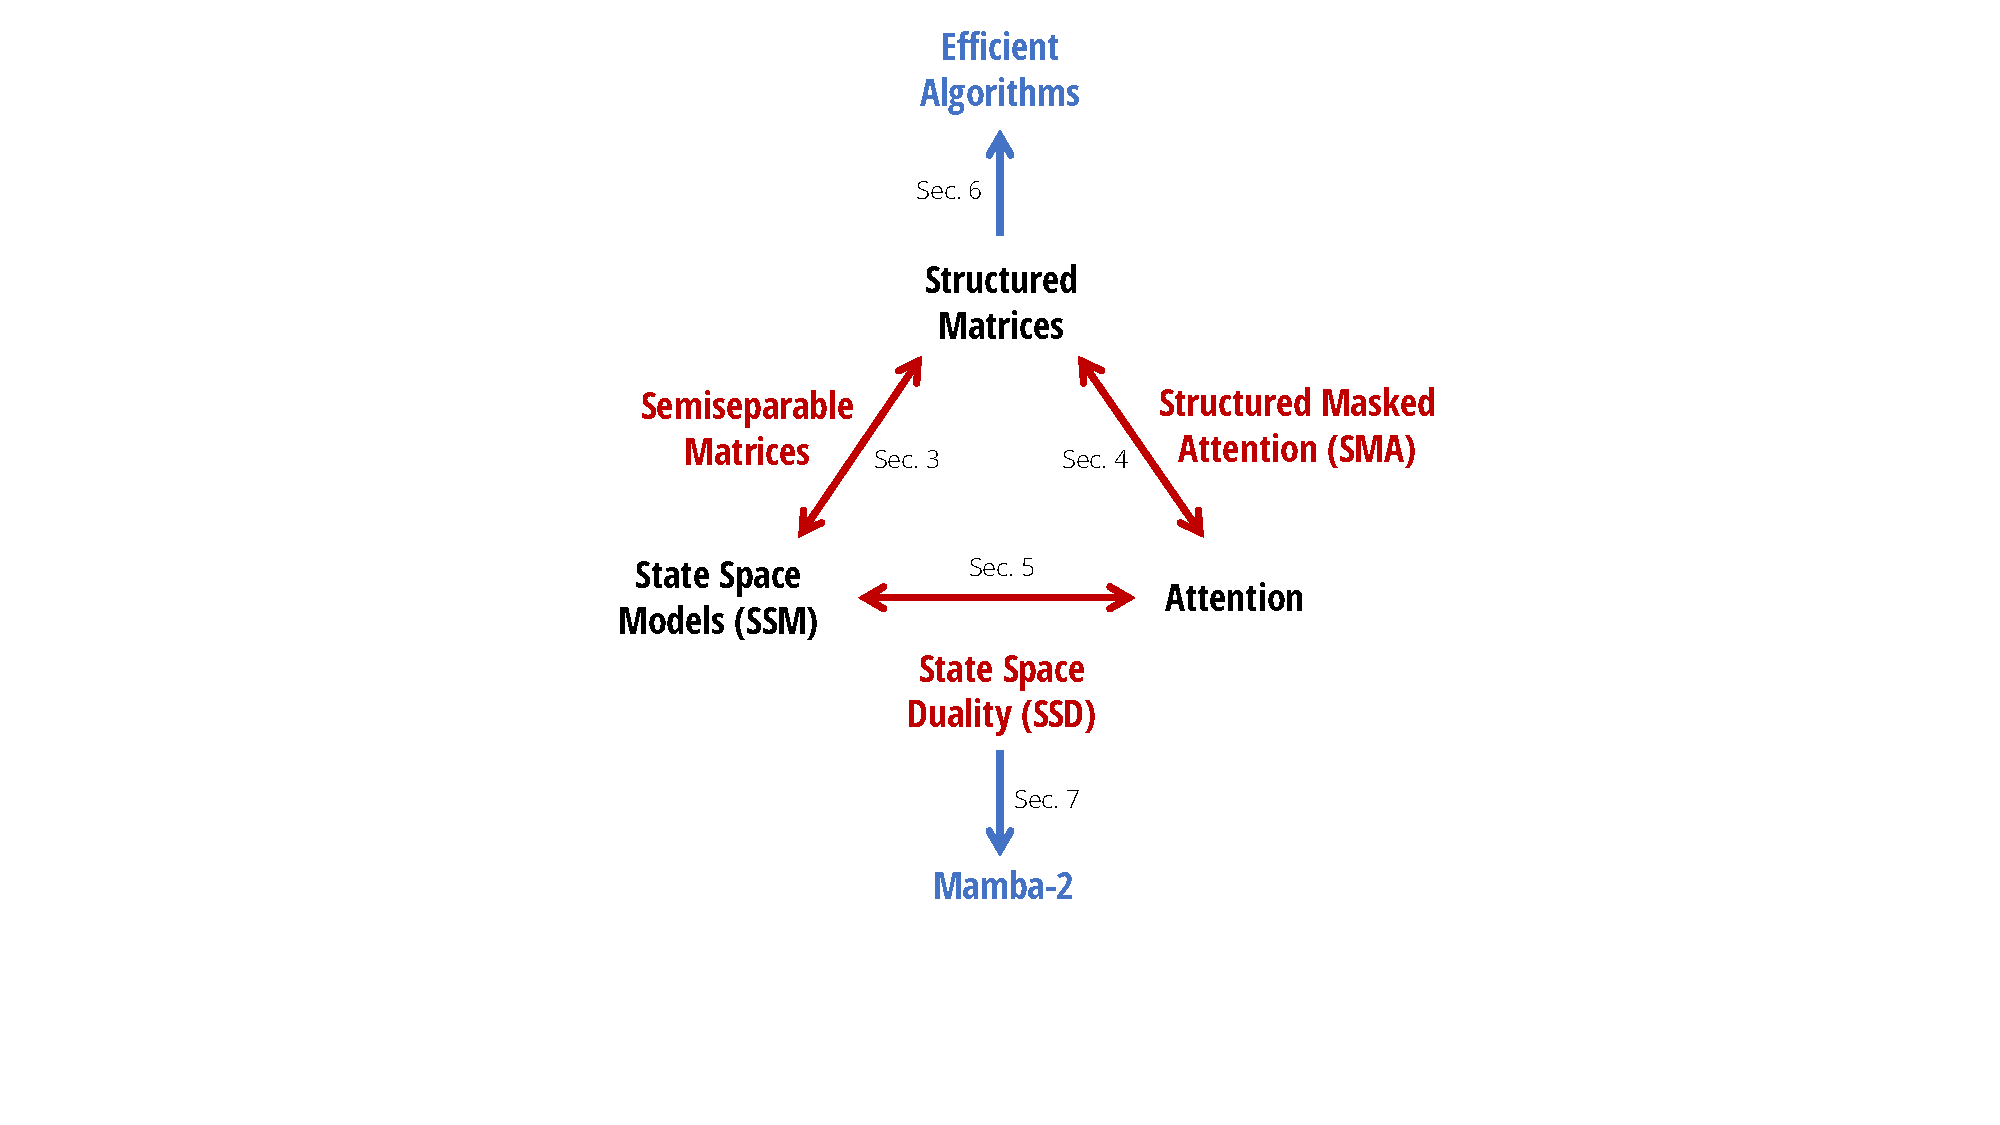
\includegraphics[width=\linewidth]{fig/ssd_roadmap.pdf}
  \end{center}
  \caption{
    (\textbf{Structured State-Space Duality}.)
    This paper fleshes out the relationship between state space models and attention through the bridge of structured matrices.
  }
  \label{fig:roadmap}
\end{wrapfigure}
}{}

\para{State Space Duality.}
Our framework connecting structured SSMs and variants of attention, which we call \textbf{structured state space duality} (SSD),
is made through the abstractions of \textbf{structured matrices}:
matrices with subquadratic parameters and multiplication complexity.
We develop two broad frameworks for representing sequence models, one as matrix transformations and one as tensor contractions, which each reveal different perspectives of the duality.
Our technical contributions include:
\begin{itemize}[leftmargin=*,itemsep=0pt,topsep=0pt]
  \item We show an equivalence between state space models and a well-studied family of structured matrices called \textbf{semiseparable matrices}\iftoggle{arxiv}{ (\cref{sec:ssm})}{}.
    This connection is at the heart our framework, revealing new properties and algorithms for SSMs. A central message of this paper is that \emph{different methods of computing state space models can be reframed as various matrix multiplication algorithms on structured matrices}.
  \item We significantly improve the theory of linear attention~\citep{katharopoulos2020transformers}.
    We first provide an incisive proof of its recurrent form through the language of tensor contractions, and then generalize it to a new family of \textbf{structured masked attention (SMA)}\iftoggle{arxiv}{ (\cref{sec:attention})}{}.
  \item We connect SSMs and SMA, showing that they have a large intersection that are duals of each other, possessing both SSM-like linear and attention-like quadratic forms\iftoggle{arxiv}{ (\cref{sec:ssd})}{}.
    \iftoggle{arxiv}{We also prove that any kernel attention method possessing a fast recurrent form must be an SSM.}{}
\end{itemize}


Beyond its intrinsic theoretical value, our framework opens up a broad set of directions for understanding and improving sequence models.

\para{Efficient Algorithms.}
First and most importantly, our framework exposes new efficient and easily-implementable algorithms for computing SSMs\iftoggle{arxiv}{ (\cref{sec:efficient})}{}.
We introduce a new \textbf{SSD algorithm}, based on block decompositions of semiseparable matrices, that takes advantage of both the linear SSM recurrence and quadratic dual form, obtaining optimal tradeoffs on all main efficiency axes (e.g. training and inference compute, memory usage, and ability to leverage matrix multiplication units on modern hardware).
A dedicated implementation of SSD is $2-8\times$ faster than the optimized selective scan implementation of Mamba, while simultaneously allowing for much larger recurrent state sizes ($8\times$ the size of Mamba or even higher, with minimal slowdown).
SSD is highly competitive with optimized implementations of softmax attention (FlashAttention-2~\citep{dao2023flashattention2}), crossing over at sequence length 2K and 6$\times$ faster at sequence length 16K.


\iftoggle{arxiv}{
\para{Architecture Design.}
One major obstacle to adopting new architectures such as SSMs is the ecosystem tailored to Transformers, such as hardware-efficient optimization and parallelism techniques for large-scale training.
Our framework allows using established conventions and techniques for attention to build a vocabulary of architecture design choices for SSMs, and further improve them (\cref{sec:architecture}).
For example, we introduce the analog of heads from multi-head attention (MHA) to SSMs.
We show that the Mamba architecture is a \textbf{multi-input SSM (MIS)} that turns out to be analogous to \textbf{multi-value attention (MVA)}, and compare other variants of Mamba with different head structures.

We also use these ideas to make slight modifications to the Mamba block, which allows tensor parallelism to be implemented (e.g. in the style of Megatron~\citep{shoeybi2019megatron}).
The main ideas include introducing grouped-value attention (GVA) head structure, and moving all data-dependent projections to occur in parallel at the beginning of the block.


}{
  \para{Mamba-2.}
  Additionally, inspired by the connection between SSMs and Transformers, we slightly modify the neural network architecture of Mamba by moving all data-dependent projections to occur in parallel at the beginning of the block. %
}
The combination of the modified parallel Mamba block, together with using SSD as the inner SSM layer, results in the \textbf{Mamba-2} architecture.
We investigate Chinchilla scaling laws for Mamba-2 in the same setting as Mamba, finding that it Pareto dominates Mamba and Transformer++ in both perplexity and wall-clock time.
We additionally train a family of Mamba-2 models at varying sizes on the Pile, showing that it matches or outperforms Mamba and open source Transformers on standard downstream evaluations.
For example, Mamba-2 with 2.7B parameters trained on 300B tokens on the Pile outperforms Mamba-2.8B, Pythia-2.8B and even Pythia-6.9B trained on the same dataset.

\iftoggle{arxiv}{
\paragraph{Systems Optimizations.}
The SSD framework connects SSMs and Transformers, allowing us to leverage a rich body of work on systems optimizations developed for Transformers~(\cref{sec:systems}).
\begin{itemize}[leftmargin=*,itemsep=0pt,topsep=0pt]
  \item For example, Tensor Parallelism (TP) is an important model parallelism technique to train large Transformer models by splitting each layer across GPUs on the same node.
    We design Mamba-2 to be TP-friendly, reducing the number of synchronization point per block by half.
  \item For very long sequences whose activations do not fit on one device, sequence parallelism has been developed for the attention blocks.
    We describe how to train SSMs in general and Mamba-2 in particular with sequence parallelism, by passing the recurrent states between devices.
  \item For finetuning with examples of different lengths, for best efficiency, Transformer requires sophisticated techniques to remove padding tokens and perform attention on variable length sequences.
    We show how Mamba-2 can be trained with variable sequence lengths efficiently, requiring no padding tokens.
\end{itemize}
}{}

\cref{sec:experiments} empirically validates Mamba-2 on language modeling, training efficiency, and a difficult multi-query associative recall task~\citep{arora2024simple}.
Finally, in \cref{sec:related}, we provide an extended related work and discuss potential research directions opened up by our framework.

Model code and pre-trained checkpoints are open-sourced at \url{https://github.com/state-spaces/mamba}.







\section{Background and Related Work}
\label{sec:back}

We begin by providing background on style mimicry and existing image-based protection methods. Then we follow with an overview of publicly available tools that enable style mimicry attacks on the video domain.

\subsection{Style Mimicry and Existing Defenses}
\label{sec:back1}
In a style mimicry attack, a bad actor finetunes a text-to-image model to
generate art in a particular artist's style without their consent. 
Since the introduction of text-to-image diffusion~\cite{sd-release,podell2023sdxl,df,novelai-update,ramesh2022hierarchical} models in 2022, style mimicry has grown significantly. There have been multiple high-profile mimicry incidents involving human artists~\cite{hollie-steal,sarah-andersen,lensa-steal,sam-steal}, and new companies are founded that focus purely on style mimicry~\cite{aigame,lexica}. AI marketplaces have also recently gained traction, with websites like CivitAI~\cite{civitai} offering over 119K ready-to-use mimicry models for people to download and use.

\para{Image-based style mimicry. } 
Style mimicry relies on finetuning pretrained text-to-image models (\eg stable diffusion) on a small set of images from a specific style~\cite{ruiz2022dreambooth,finetune-c,gal2022image}. The quality of these images greatly impacts the mimicry result, and thus, attackers often scrape high quality images from artists' websites and online galleries~\cite{hollie-steal,sam-steal}. In practice, a bad actor does not need many (less than 20 images~\cite{shan2023glaze,gal2022image}) in order to successfully generate arbitrary artwork from a victim artist's style. Because of the risk of image-based mimicry, many artists choose to reduce the amount of art they post online~\cite{aiprotest}, reduce the quality of any posted art~\cite{lowres}, and apply protection (discussed in details below) on this artwork~\cite{shan2023glaze}. 

\para{Protecting images from style mimicry. } 
Existing work (Mist~\cite{mist}, Anti-Dreambooth~\cite{antidb}, and Glaze \cite{shan2023glaze}) has 
proposed methods that leverage clean-label poisoning~\cite{saha2020hidden, turner2018clean, zhu2019transferable} to prevent style mimicry. At a high level, these systems add small optimized perturbations to image artwork that modifies the perturbed image's feature space representation without altering its content. The altered feature space representation prevents models from learning the correct artistic style. In general, these protection tools calculate the perturbation $\delta_x$ for an image $x$ using the following objective: 

\secspace
\begin{eqnarray}
   &\min\limits_{\delta_x} Dist\left( \Phi(x + \delta_x), \Phi(T)\right),  \label{eq:cloakopt}\\
  & \text{subject to } \; |\delta_x|< p, \nonumber
\end{eqnarray} 

where $\Phi$ is a generic image feature extractor from a public text-to-image model, $Dist(.)$ computes the distance between two feature representations, $|\delta_x|$ measures the perceptual perturbation caused by protection, and $p$ is the perceptual perturbation budget. $T$ is 
a ``target image'' that the perturbation $\delta_x$ is optimized towards, such that $x + 
\delta_x$ resembles $T$ in feature space while being visually identical to $x$. Mist~\cite{mist} extends the optimization objective across the entire diffusion process, including gradient computations through the randomized diffusion denoising process. By default, Mist uses a predefined black and white patterned image as its target with the goal of producing chaotic patterns in generated images. Anti-DB (Anti-Dreambooth)~\cite{antidb} is most similar to Mist, but modifies the optimization objective to specifically target Dreambooth~\cite{ruiz2022dreambooth} text-to-image models. There, they find that training surrogate models alongside computing image perturbations results in stronger protection, though it incurs additional computation time. Glaze~\cite{shan2023glaze} introduces input-specific target images by performing style transfer on the input image using a contrasting artistic style. This method preserves the overall content of the input image, while changing mainly the style, which the authors argue leads to more robust protection. Glaze then attacks the image encoder of a diffusion model as detailed above. 

These protection tools have been positively received by the artist community,
with Glaze having been downloaded at least 2.3 million
times~\cite{shan2023glazewebsite}. While these systems are typically too
computationally expensive for artists, efforts have been made to improve
accessibility~\cite{mistgithub, shan2023webglaze}. Since these systems are
free and increasingly available, images may no longer be a viable data source
for attackers to access artwork for fine-tuning text-to-image models. 

Video protection, on the other hand, has yet to be explored. Computation time per image is already limiting for many artists, and applying the same algorithms to all frames would be many times more costly. Yet, videos represent a significant source of data, incentivizing attackers to explore publicly available video art, such as short animation, movies or video game trailers etc..

Until recently, most style mimicry models are trained on still images. This 
is no longer the case today because 1) artists are increasingly more reluctant to post their 
work on the Internet~\cite{aiprotest}, 2) existing defenses (\S\ref{sec:back1}) are effective at protecting still images against mimicry, 3) video frames offer a significantly more diverse range of images compared to still images. 

\para{Video content is a promising source for mimicry. } 
Video content (\eg game trailers, anime, short videos, documentary, ads) provides promising alternative data sources for two reasons. First, video contents often offer a more diverse (3D) shots of an object or style, \eg rotating shot of an object, panning across a scene. These diverse viewpoints 
enable models to better learn the content during the training process~\cite{videomotivate}. Second, there are significantly more video frames compared to still images and many of the videos contain unique art styles/characters. The entire Internet produces around 3.2 billions still images daily~\cite{manyvideos}, while YouTube alone sees over 271,000 hours of videos (\ie around 29 billions video frames) uploaded per day. Specifically, gaming companies and animation studios often use short videos as a way to promote new games, characters, and movies. Movie clip compilations and trailers are readily available on YouTube~\cite{movietrailers}, while video game companies like Riot and Mihoyo frequently post teasers and trailers showcasing new playable content, or highly anticipated characters~\cite{genshintrailer, leaguetrailer}. These videos are filled with original artwork, and contain image frames that are prime targets for style mimicry. 

\para{Video-based mimicry in the real-world. } 
Style mimicry using video content has already occurred in the real-world. Bad actors have created and distributed software that generates high quality text-to-image datasets from online videos. One GitHub tool~\cite{anime2sd} automates the process of downloading (\eg torrenting) Japanese Anime episodes and extracting high quality frames of desired characters. Another option~\cite{civitai-video} advertised on CivitAI does the same, with the additional capability of scraping frames from screencap websites such as FanCaps~\cite{fancaps}. These tools demonstrate that there already exists sophisticated technology aimed at creating text-to-image datasets from original video content. 

We also provide our own examples of this threat. We download and extract high quality frames from YouTube videos and train style mimicry models on them (Figure~\ref{fig:style-mimicry-scenario}). Figure~\ref{fig:style-mimicry-baseline} shows some examples of extracted video frames as well as mimicry results generated by the style mimicry model. We include human evaluation of the success of these style mimicry images later using user studies with both artists and the general public in \S\ref{sec:eval}. 

While there has been recent developments in text-to-video~\cite{videoworldsimulators2024} and image-to-video models~\cite{blattmann2023stable}, we leave them as a topic for future work, and focus solely on text-to-image mimicry where the source of data originates from video content. 


\secspace
\section{Style Mimicry Attacks on Extracted Video Frames}
\label{sec:threat}

Our work considers a previously overlooked variant of the style mimicry
attack, where an attacker extracts individual frames from a video to build
image-based style mimicry models. Next, we introduce the threat model and
consider the limitations of a baseline defense that applies existing
image-based protection tools to individual video frames.

\secspace
\subsection{Threat Model}

\para{Artist/Video creator. } Artists want to share their video 
content online while disallowing unauthorized mimicry using these video frames. 
Artists seeks to protect their video by applying small 
pixel perturbations on the video frames. Following the assumptions made by existing defenses against style mimicry~\cite{shan2023glaze}, we
assume the artists: 
\begin{packed_itemize} 
    \item have access to moderate computing resources (\eg consumer-grade GPUs) commonly used for video rendering; 
    \item add perturbation to video frames before posting videos online; 
    \item have access to some public feature extractor (\eg open-source models such as Stable Diffusion).
\end{packed_itemize}

\para{Attacker. } The attacker's goal is to build a \textit{text-to-image} model
that is able to generate images in the style of the victim artist. We assume the 
attacker 
\begin{packed_itemize} 
\item has access to videos from the victim and leverages frames from
these videos for mimicry; 
\item has significant computational power; 
\item has full access to pretrained, benign text-to-image base models. 
\end{packed_itemize}
Note that our work focuses on text-to-image mimicry, where the attacker's goal
is to {\bf generate images}. We leave text-to-video 
mimicry using video contents to future work. 

\begin{figure}[t]
    \centering
    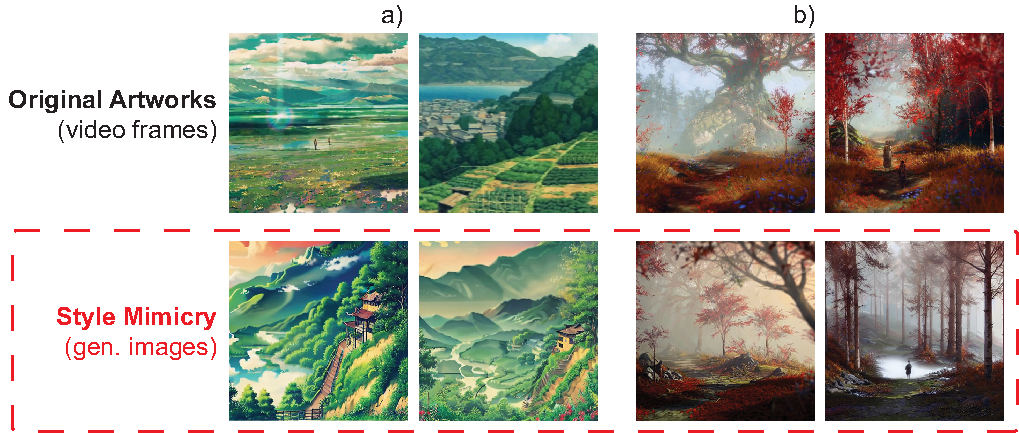
\includegraphics[width=1\columnwidth]{plots/clean-style-mimicry-eps-converted-to.pdf}
    \vspace{-0.2in}
    \caption{Style mimicry on clean video frames successfully mimics style of original video.}
    \label{fig:style-mimicry-baseline}
  \end{figure}
\subsection{Style Mimicry Leveraging Video Frames}

\subsection{A Naive Defense and Its Limitations}
\label{subsec:limitations}

Given the existence of existing tools designed to disrupt art style
mimicry~\cite{shan2023glaze,mist,antidb}, a straightforward solution to
protect video imagery is to simply apply existing protection to each and
every frame of a video.  As discussed in \S\ref{sec:back}, these defenses add
highly-optimized perturbations on each image (a video frame in our case),
misleading the mimicry model to perceive each protected frame as an image with a
completely different style.

Unfortunately, this ``naive'' application of anti-mimicry tools in the video
context has multiple drawbacks, the most critical of which is vulnerability
to a temporal-based adaptive countermeasure.

\para{Vulnerability to countermeasures based on temporal similarity.}  When
applied on individual video frames without coordination, existing protection
methods become vulnerable to advanced countermeasures that exploit
visual similarity across consecutive video frames.

Existing anti-mimicry tools treat each input image independently, with a
randomized component in their generation of perturbation targets for each
image. That means even two runs on the same input image will likely output
two different set of pixel changes. With this in mind, an adaptive mimicry
attack could take several consecutive frames, whose original pixel values are
highly similar, and use them against each other to try to cancel out the
pixel changes made by the protection tools.  An``averaged'' or
``smoothed'' frame generated this way would have much weaker residue
protective perturbations, and would provide a good estimate of the
actual visual feature (i.e. style) carried by the original (unperturbed)
video frames.  An attacker can then use these frames to train a
mimicry model. In \S\ref{sec:eval-limitations}, we provide a detailed study to
validate and quantify this significant vulnerability.


\para{Other limitations: computation and video quality degradation.} The
naive application of protection tools leads to two other challenges. First,
computing independent protection filters on each video frame is
computationally very expensive.  Existing protection tools
(Glaze~\cite{shan2023glaze}, Mist~\cite{mist} and Anti-DB~\cite{antidb}) can
takes up to $\tau=1.5$ minutes to protect a single frame for moderate
GPUs. Protecting a 1 minute video at 30fps (1800 frames) would take 45 hours.
Second, the protective pixel level perturbations are computed independently per
frame and hard to detect on a still image. But when played in a video
sequence, these perturbations cause noticeable flickering effects that
degrade the video quality and viewer experience.

\secspace
\section{An Adaptive Mimicry Attack} 
\label{sec:eval-limitations}
In this section, we design, implement and evaluate an adaptive mimicry attack
designed to bypass the naive protection method described in
\S\ref{subsec:limitations}. 

It is made possible by the fundamental {\em temporal consistency} inherent to
all video content. Here, we propose {\em Perturbation Removal Attacks} (PRA)
that leverage temporal consistency to remove protective perturbations on
video frames, and present results measuring their efficacy using both
automated metrics and human feedback.

\secspace
\subsection{Perturbation Removal}

For naively protected video sequences, we develop an adaptive mimicry attack
that uses perturbation removal methods (PRM) to recover images that closely
approximate the original, unperturbed video frames. These are then used to
successfully train an image-based style mimicry model.  As such, for any
video sequence, a PRMs behaves like a frame extraction tool.

\para{``Combining'' consecutive frames.} PRMs remove protective perturbations
by combining multiple consecutive video frames (that share high visual
similarity) into a single frame. Intuitively, combining highly similar frames
will generally preserve the common pixel values inherited from the original
unprotected frames, while reducing or removing the pixel value changes made
by protective tools.  With this in mind, we consider three PRM approaches that
employ different ``combining'' functions across video frames.

\begin{packed_itemize}
\item \textbf{Selective Pixel Averaging} -- This approach generates a
  combined image out of consecutive frames, where each pixel is the average
  of the corresponding pixel values across the set of frames. This
  pixel-level ``averaging'' function ``smooths'' out the protective
  perturbations. Pixel averaging can be limited to more static regions and
  avoid pixels that capture motion across the frames. 
\item \textbf{FILM} -- Frame Interpolation for Large Motion
  (FILM)~\cite{reda2022film} is a neural network designed to generate
  temporally smooth videos from disjoint frames. We apply FILM to multiple
  perturbed frames from the same scene to reconstruct high quality images
  that closely resemble the original unperturbed frames, but don't retain
  perturbations from either input.
\item \textbf{Linear Interpolation} -- Linear interpolation is
  a technique for generating intermediate data points between a set of known
  points. Like the other approaches, pixel-level linear interpolation 
  across frames exploits lack of consistency between consecutive
  perturbations.
\end{packed_itemize}

\para{Implementing adaptive attacks.} We implemented 3 adaptive mimicry attacks, each
using one of the frame-aggregation approaches described above. In the rest of
this section, we present detailed results on all 3 adaptive attacks. The key
takeaway is that pixel averaging significantly outperforms the
alternatives. For brevity, we move implementation details of the other two
attacks to Appendix \ref{app:detailed-perturbation-removal}, and only provide
implementation details for the pixel averaging below. 

\begin{figure}[t]
  \centering
  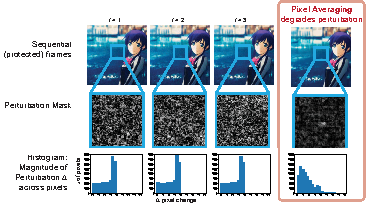
\includegraphics[width=1\columnwidth]{plots/pixel-averaging-scenario-04-eps-converted-to.pdf}
  \vspace{-0.2in}
  \caption{Averaging pixel values across highly similar consecutive frames
    successfully degrades the randomized protection pixel shifts across
    frames and largely restores the original unprotected frame. }
  \label{fig:pixel-averaging-attack}
\end{figure}

\emph{Pixel Averaging} approximates the original unprotected frame by
averaging pixels across highly similar consecutive frames (see
Figure~\ref{fig:pixel-averaging-attack}). Pixel level differences between
consecutive frames come from two sources: 1) natural changes between video
frames which we call \textit{movement}, and 2) differences in pixel changes
added by protective tools (\textit{perturbations}). Protective tools seek to
minimize visual impact, so the large majority of perturbation values are
constrained within a specific value. Thus an attacker can examine two
consecutive perturbed frames, and identify the source of each pixel
difference by filtering using a simple threshold ($\epsilon_p$). A well
chosen $\epsilon_p$ will separate pixel differences due to movement
($>\epsilon_p$) from pixel differences from protective tools
($<\epsilon_p$). The attacker measures pixel differences ($\Delta_p$) between
consecutive frames and only averages regions ($0 < \Delta_p <
\epsilon_p$). In practice, $\epsilon_p$ can easily be identified empirically
as a transition point between two levels of region sizes. In our tests, we
experimentally test pixel averaging across $n$ consecutive frames, and find
the best results around $n=5$.  We measure the quality of frames using CLIP
Aesthetic predictor~\cite{schuhmann2022laion} and perturbation removal using
metrics described in the following section. We show detailed results of the
tradeoff between perturbation removal vs. image quality in the appendix.

\subsection{Experimental Setup and Metrics}
To validate the efficacy of multiple perturbation removal methods, we add
naive protection to short scenes on an independent, per-frame basis. We then
test the adaptive mimicry attack by using each PRM to extract unprotected
frames from each video scenes. We compare different PRMs by measure the
amount of image level differences in the perturbations before vs. after our
attack using several automated metrics. We also measure end-to-end
success of the adaptive mimicry attack by training models on
extracted frames, and conducting a user study to gather human
feedback.

\para{Applying naive protection to all frames.}  We experiment on 5 diverse
datasets containing realistic videos of scenery and human actions, artistic
style videos, and video game style videos. We implement each of 3 protection
tools, Mist, Anti-DB, and Glaze.  For each scene, we identify and extract
scenes of highly similar frames, and apply ``naive protection'' by applying
each of 3 protection tools to each frame in selected frames. We apply each
PRM to the naively protected images to attempt to recover a good estimation
of the original images. We then compare original, naively protected, and
attacked naively protected images to each other.
As we show below, pixel-averaging significantly outperforms FILM and linear
interpolation in pixel level metrics.

\para{Performing style mimicry.} We perform style mimicry attacks under 3
``perturbation scenarios'': training mimicry models on 
clean (unperturbed) frames, frames protected by ``naive protection,'' and
frames extracted by adaptive attack following ``naive protection.''  Due to
high computation costs (multiple days per scene), we only compute end-end
results for the Pixel Averaging attack (shown to be strongest in pixel level
metrics above).
For each perturbation scenario, we chose ~30
scenes from a video, select (or extract) one image from each scene,
and train mimicry models on this set.  Further details on mimicry attack
configurations are in \S\ref{sec:eval}.

\para{Evaluation metrics.}  We evaluate the strength of perturbation removal
methods using pixel level metrics (Mean Pixel Difference and Latent $L_2$ Norm). 
We evaluate end-to-end results on style mimicry using human feedback
(User Study). We briefly describe these metrics below, and give more details later in
\S\ref{sec:eval}.

\begin{packed_itemize}
\item{\em Latent $L_2$ Norm.} We employ the image encoder used in diffusion models
  to calculate image representations of perturbed and non-perturbed (original)
  frames, and then calculate the $L_2$ distance between them as a measure
  of proximity between two images. Thus, a successful perturbation removal
  would minimize the latent $L_2$ norm, while a robust system should maintain a
  high latent $L_2$ norm.

\item{\em Mean Pixel-Difference.}  We measure differences between images at a
  pixel level, motivated by the $l_{inf}$ bounded pixel changes that all
  protection tools (Mist, Anti-DB, Glaze) use to limit visual artifacts. We
  define Mean Pixel Difference (MPD) as the average of all pixel differences
  between a perturbed image and clean image. Similar to the latent $L_2$ norm, 
  a higher MPD signals higher protection.

\item{\em Human feedback.}  We perform a user study to evaluate the success
  of adaptive mimicry attacks, by asking participants to look at images
  produced by a mimicry model, and compare it to original video frames.  We
  ask participants to rate the success on a 5-level Likert scale (ranging
  from ``not successful at all'' to ``very successful''). Following existing
  work, we define protection success rate (PSR) as the percent of
  participants who rated the style mimicry as ``not very successful'' or
  ``Not successful at all.''
\end{packed_itemize}

\begin{figure}[t]
  \centering
  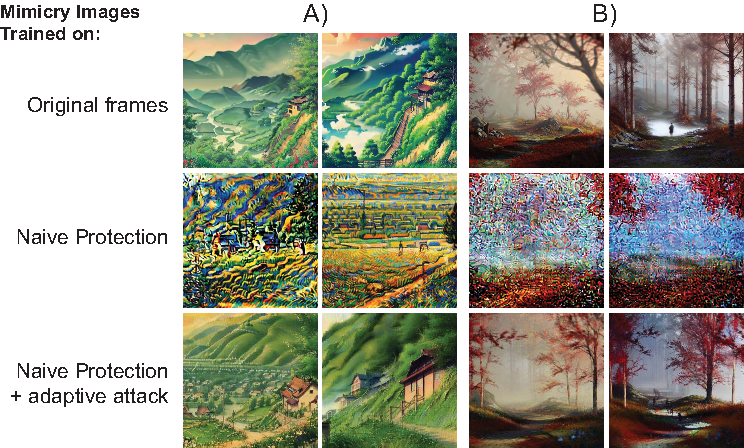
\includegraphics[width=1\columnwidth]{plots/pixel-avging-success-eps-converted-to.pdf}
  \vspace{-0.3in}
  \caption{Visual examples of adaptive mimicry attack. Three rows of
      mimicry images generated by models trained on 1) original video frames,
    2) video frames protected naively, and 3) video frames recovered after
    perturbation removal using pixel averaging.}
  \label{fig:style-mimicry-attacked}
\end{figure}

\begin{table}[t]
  \centering
    \resizebox{0.5\textwidth}{!}{
    \centering
\begin{tabular}{c|cccc}
 Protection Tool  & Protected          & Pixel Avg                   & FILM Interpolation & Linear Interpolation \\ \hline
  Glaze          & 390.05 $\pm$ 25.17 & \textbf{295.55 $\pm$ 52.02} & 391.51 $\pm$ 62.86 & 355.58 $\pm$ 44.38   \\
  Mist           & 474.87 $\pm$ 42.14 & \textbf{334.62 $\pm$ 56.72} & 437.78 $\pm$ 64.89 & 411.27 $\pm$ 51.89   \\
  Anti-DB        & 405.17 $\pm$ 37.55 & \textbf{283.41 $\pm$ 58.99} & 378.43 $\pm$ 67.34 & 352.10 $\pm$ 52.30  
  \end{tabular}
  }\caption{Latent $L_2$ Norm between original frames, protected frames
    and protected frames after perturbation removal.}
\label{tab:loss-removal-results}
\vspace{-0.2in}
\end{table}


\begin{table}[t]
  \centering
    \resizebox{0.5\textwidth}{!}{
    \centering
\begin{tabular}{c|cccc}
  Protection Tool & Protected          & Pixel Avg                   & FILM Interpolation & Linear Interpolation \\ \hline
  Glaze          & 111.30 $\pm$ 12.94 & \textbf{90.04 $\pm$ 14.13}  & 97.83 $\pm$ 13.73  & 96.16 $\pm$ 14.47    \\
  Mist           & 121.25 $\pm$ 9.48  & \textbf{107.10 $\pm$ 16.33} & 112.99 $\pm$ 14.36 & 113.03 $\pm$ 15.46   \\
  Anti-DB        & 124.86 $\pm$ 8.93  & \textbf{103.75 $\pm$ 17.70} & 110.29 $\pm$ 15.52 & 110.39 $\pm$ 16.42  
  \end{tabular}
  }\caption{Mean Pixel Difference between original frames, protected frames,
    protected frames after perturbation removal.}
\label{tab:pd-removal-results}
\vspace{-0.2in}
\end{table}


\subsection{Adaptive Mimicry Results}

Next we present results of our experiments on the adaptive attack.

\para{Similarity of recovered frames to original frames.} We compare
{\em latent $L_2$ norm} 
between the original frames, the protected frames, and protected frames after
protection removal.  Table~\ref{tab:loss-removal-results} shows FILM to
have minimal impact, and that Pixel averaging does the best to minimize loss
for the recovered frame, suggesting that it is closer to the original frame
in the feature space.

We also compare {\em mean pixel differences} between the original
frames, protected frames, and protected frames after protection removal.
Table~\ref{tab:pd-removal-results} shows that again, pixel averaging method
outperforms against all protection tools, and minimizes the pixel differences
between the extracted frame and the original. 

\para{Style mimicry attack on recovered images.}  Finally, we use a user
study to evaluate the end-to-end success of the adaptive mimicry attack using
pixel-averaging to overcome a per-frame application of protection tools.
Table~\ref{tab:user-study-removal-results} shows that users agree, the
adaptive mimicry attack with pixel averaging basically produces mimicry
results similar to mimicry on original unprotected video frames (PSR baseline
value of 17.65 for unprotected video frames).
Figure~\ref{fig:style-mimicry-attacked} shows samples of mimicry images from
models trained on original frames, protected frames, and protected frames
under adaptive attack. Clearly the adaptive attack is able to bypass
protection and restore mimicry success.

These results validate our concerns, that a naive, frame by frame application
of protection tools to videos is insufficient to prevent image mimicry. We
need to extend these anti-mimicry tools to restore their protection in the
video domain.

\secspace

\section{Protecting Video Imagery with \system{}}
\label{sec:method}
We have identified that video imagery is susceptible to style mimicry attacks
despite existing protection in image space (\S\ref{sec:eval-limitations}).
Although current protection tools are effective for 2D art, they are no longer robust
to adaptive adversaries in the video domain. In this section, we
develop \system, a framework that extends image-based protection tools to the video
domain, resulting in improved robustness against adaptive adversaries as well
as lower computation costs and improved video quality for protected videos.

\begin{table}[t]
  \centering
    \resizebox{0.4\textwidth}{!}{
    \centering
\begin{tabular}{c|cc}
  Protection Tool & Protected        & Protected + Pixel Averaging                 \\ \hline
  Glaze          & 70.59 $\pm$ 1.05 & \textbf{23.76 $\pm$ 1.14} \\
  Mist           & 62.90 $\pm$ 1.11 & \textbf{25.34 $\pm$ 1.14} \\
  Anti-DB        & 59.28 $\pm$ 1.18 & \textbf{22.62 $\pm$ 1.15} 
  \end{tabular}}
  \caption{Human feedback (Protection Success Rate) shows perturbation
    removal can significantly reduce effects of protection tools 
    against style mimicry attacks. Note baseline PSR for original,
    unprotected frames is 17.65 $\pm$ 1.10.}
\label{tab:user-study-removal-results}
\vspace{-0.2in}
\end{table}

\begin{figure*}[t]
  \centering
  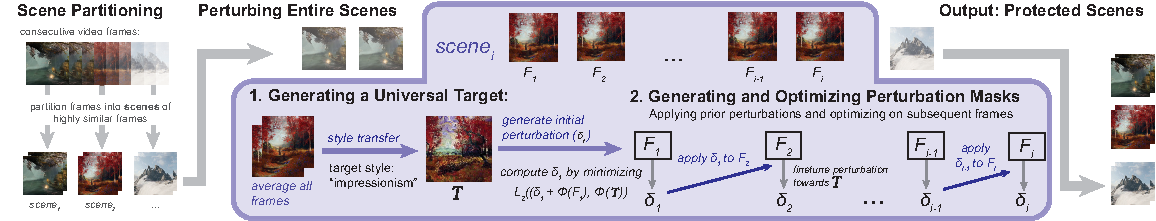
\includegraphics[width=1\textwidth]{plots/system-design-02-eps-converted-to.pdf}
  \vspace{-0.25in}
  \caption{\system~ partitions videos into scenes by measuring average pixel difference. Each scene is perturbed using a two-part process: 1) A target image ($T$) is computed by averaging all frames and style transferring to a 'target style' 2) Perturbations are iteratively applied and optimized by minimizing latent $L_2$ norm between $T$ and the perturbed frame.}
  \label{fig:system-design}
\end{figure*}


\subsection{Design intuition} 

\para{Challenges of existing perturbation systems.} Existing perturbation
systems do not take into account the threat of an adversary gaining access to
highly similar or even identical frames that are protected with completely
independent perturbations.  These systems independently optimize separate
protection perturbations for each frame.

This optimization process includes 1) generating a \textit{random} target latent
tensor, and 2) perturbing the original image by optimizing the 
image towards the selected target.  The choice of target significantly
impacts the pixel level perturbations on an image. Current systems choose
targets by generating a latent representation of the original image,
introducing noise, and then employing denoising autoencoders.  This
randomness (\ie non-linearity) is desired for image-based protection, making
it more challenging to reverse engineer or remove the perturbations. However,
it also leads to each perturbation mask being entirely unique; disregarding
the temporal redundancy present in the original frames. This in turn gives
rise to effective countermeasures that remove the protection
(\S\ref{sec:eval-limitations}).

\para{Intuition.}
Our key intuition is that if we can create very similar perturbations on
similar underlying frames, we can nullify the adversaries ability to exploit
duplicity in frames. With this in mind, there are two simple options for
perturbing a scene of similar frames. The first option is to re-use the same
perturbation for the entire scene. Re-using the same perturbation is robust
to pixel averaging attacks, but frame-specific protection weakens after
small levels of movement in frames.

A second option is that if we can chose very similar targets (that guide the
optimizing of perturbations) for similar frames, we can increase the
consistency between perturbations. We find that re-using a single target
tensor throughout a scene leads to very similar perturbations, but also makes
frames less robust to style mimicry. This is because the perturbation
optimization algorithm is not able to customize the embeddings of different
frames to the same degree as it does for the original frame the
target tensor was generated from. Thus our goal is to 1) divide 
videos into scenes that can share a \textit{universal} target, 2) generate
this ``universal target'' for each scene, and 3) optimize perturbations on
subsequent frame to maximize protection against mimicry.

\subsection{System Design}

Figure~\ref{fig:system-design} describes our pipeline for generating robust,
protected videos by partitioning them into scenes, generating a target image
for each scene, and then optimizing the perturbations on each frame towards
its respective target. 

\para{Scene partitioning.}  We want to pinpoint sections of videos where
using different perturbations might leave frames vulnerable to averaging
attacks. We split videos into distinct scenes based on frame similarity, and
considered existing scene partitioning algorithms and
tools~\cite{pyscenedetect}. Note that we require all frames in a scene to be
similar enough to share a single ``perturbation target.'' This is a stronger
constraint than most prior definitions for a ``scene,'' leading us to
implement our own algorithm. We split scenes based on the mean pixel
difference between two consecutive frames $F_i$ and $F_{i-1}$, defined
by \secspace
\begin{equation}
 \frac{Pixel(F_i, F_{i-1})}{N}< \epsilon_{scene}\label{eq:mean_pixel_diff}
\end{equation}
where $N$ is the number of pixels per frame and $Pixel(.)$ calculates
the pixel difference between two frames, and $\epsilon_{scene}$ is a
parameter for scene partition. 

\para{Generating a universal target.}  To create consistency between
consecutive perturbations, we compute a single target image for all frames in
a scene. This means that the target embedding needs to be close enough the
embeddings of each frame in the scene, so that it can correctly guide each
individual optimization. We test several approaches to generating the target
tensor: 1) using the middle frame from the scene as base image, 2) generating
image embeddings of each frame in the scene, calculating the centroid of
these embeddings as base image, and 3) averaging all frames together as base
image. We measure latent $L_2$ norm distance between the embedding of each unique frame in a
scene and the target tensor, and find that averaging all frames in a scene
leads to a target that is consistently the closest distance across all frames
(Figure~\ref{fig:target-selection-algorithm-results} in Appendix).

Specifically, we compute a style transferred target image $T$ from the averaged
image, like prior work~\cite{shan2023glaze}. We select a video-specific
prompt to guide the style transfer, for example: \textit{Japanese Anime} videos
use ``impressionist painting by Van Gogh'' as the target style.

\para{Generating and optimizing perturbation masks.}  We consider several
factors when computing perturbations: maximizing protection, robustness
against perturbation removal attacks, and finally, reducing computation
costs. We balance re-using perturbations on subsequent frames \textit{which
  enhances robustness against removal attacks} with optimizing or recomputing
perturbations \textit{which maintains high protection levels against mimicry
  attacks}. Protection success is achieved by reducing loss between a
perturbed image and target image. We develop our algorithm for perturbing a
scene as follows:

\if 0

\begin{packed_itemize}
  \item We compute $T_s$ using all frames in a scene (described above).
  \item The first frame $F_1$ is perturbed normally, optimizing towards
    $T_s$.
  \item For following frames, we first consider the current perturbation mask.
  If we measure the distance $L_2(F_2,T_s)$ and 
  is close enough to $L_2(F_1,T_s)$, we allow reusing perturbation on this
  frame. If not close enough, we continue optimization process on the reused
  perturbation for $F_2$ until loss decreases enough. Alternatively, if loss
  surpasses our second threshold we recompute perturbation fully. Because the
  perturbation is generated using the same target image, the system maintains
  high consistency between perturbations.
\item Repeat this process for each consecutive frame in order, using the
  latest updated perturbation mask as the base.
\end{packed_itemize}

\fi

\begin{packed_itemize}
  \item Given the current scene and its corresponding $M$ frames $\{F_i\}_{i=1}^{M}$, compute the target frame $T$ (described above).
  \item For the first frame $F_1$, compute an image-based perturbation
    $\delta_{i}$ from scratch, optimizing towards the target frame
    $T$, as defined by eq. (\ref{eq:cloakopt}). 
   \item For each subsequent frame $i$ ($i=2..M$), first compute
     \begin{equation}
       d_i=|L_2(\Phi(F_i+\delta_{i-1}), \Phi(T)) -
       L_2(\Phi(F_{i-1}+\delta_{i-1}),\Phi(T))| \label{eq:vg}
     \end{equation}
     where $\Phi(.)$ is 
     the feature extractor used to convert an image into a
     latent embedding, $L_2$ is the L2
     distance between the two embeddings. Compute  $\delta_{i}$, the perturbation for
     $F_i$  as follows:
     
     \begin{itemize}
     \item $d_i\leq\tau_1$: reuse the previous frame's perturbation,
       i.e. $\delta_{i}=\delta_{i-1}$;
     \item $\tau_1<d_i\leq\tau_2$: compute $\delta_{i}$ by
      performing perturbation optimization towards $T$ starting from
      $\delta_{i-1}$;
      \item $d_i > \tau_2$, compute $\delta_{i}$ from scratch.
    \end{itemize}

\end{packed_itemize}
Here we note that because the
  perturbation is generated progressively using the same target image
  $T$, the system is able to maintain 
  high consistency between perturbations.
  

\para{Setting $\tau_1$ and $\tau_2$.}
\label{subsec:system-parameters}
Our system applies two thresholds $\tau_1$ and
$\tau_2$ to guide the perturbation computation.  We use grid search
to identify proper values that balance robustness and computational
efficiency in all videos. In practice, content creators can perform a benchmark on their own videos to select thresholds that best balance their robustness and efficiency requirements. Further details on our grid search is located in the Appendix.

\section{Evaluation}
\label{sec:eval-cloak}

In this section, we evaluate \system's efficacy in protecting artists from
style mimicry. We first describe the datasets, models, and experimental
configurations used in our tests. Then we present the results of \system's
protection in a variety of settings. Due to \system's highly visual nature,
we evaluate its performance using both direct visual assessment by
\textbf{human artists} in a user study, and \textbf{automated metrics} (see
\S\ref{sec:metrics} for details).

\para{Summary of results.} Over $93\%$ of artists surveyed believe \system{}
effectively protects artists' styles from AI style mimicry
attacks. Protection efficacy remains high in challenging settings, like when
the mimic has access to unprotected artwork. \system{} also achieves high
protection performance against a real-world mimicry-as-a-service platform. Of
our $1156$ artist participants, over $92\%$ found the perturbations
introduced by cloaking small enough not to disrupt the value of their art,
and over $88\%$ would like to use \system{} to protect their own artwork from
mimicry attacks.

\secspace
\subsection{Experiment Setup}
\label{sec:cloak-setup}

\para{Mimicry dataset. } We evaluate \system's performance in protecting the styles of the following two groups of artists: 

\vspace{-0.2cm}
\begin{packed_itemize}
\item {\em Current artists}: $4$ professional artists let us use their
  artwork in our experiments. These artists have different styles and
  backgrounds (\eg full-time/freelancers, watercolor painters/digital
  artists, well-known/independent). Each provided us with between $26$ to
  $34$ \textit{private} original art pieces for our experiments. We use
  perceptual hashing~\cite{ke2004efficient} to verify that none of these are
  included in existing public datasets used to train generic text-to-image
  models (e.g.~\cite{schuhmann2022laion,changpinyo2021conceptual}).  

\item {\em Historical artists}: We also evaluate \system{}'s protection on
  $195$ historical artists (\eg van Gogh, Monet) from the WikiArt
  dataset~\cite{saleh2015large}. The WikiArt dataset contains 42,129 art
  pieces from $195$ artists. Each art piece is labeled with its genre (\eg
  impressionism, cubism). We randomly sampled $30$ art pieces from each
  artist to use in style mimicry attacks. Generic text-to-image models found
  online have been trained on some artwork from these artists. Using this art
  simulates a more challenging scenario in which a famous artist attempts
  to disrupt a model that already understands their style.
\end{packed_itemize}
\vspace{-0.2cm}

\para{Mimicry attack setup. } We recreate the strongest-possible mimicry
attack scenario, based on techniques used in real-world mimicry
incidents~\cite{ruiz2022dreambooth,sam-steal,hollie-steal},
that works as follows. First, we take art pieces from the victim artist $V$
and generate a text caption for each piece using an image captioning
model~\cite{luo2022vc}. \revise{The pretrained image captioning model generates a short 
sentence to describe the image. We found that this model can correctly caption protected images (examples in Figure~\ref{fig:data-examples}), likely because \system{} focuses on perturbing style features while the captioning models focus on image content.} Then, we append the artist's name to each caption,
\eg ``mountain range \textit{by Vincent van Gogh}''. Finally, we fine-tune a pre-trained generic text-to-image model
(details below) on the caption/image pairs. 

We use $80\%$ of the art pieces from the victim artists to fine-tune models
that mimic each artist's style, reserving the rest for testing. We fine-tune
for $3000$ optimization steps, which we find achieves the best mimicry
performance (Figure~\ref{fig:success-iter} in Appendix). We then use the
fine-tuned, style-specific model to generate mimicked artwork in style of
each victim artist. We query the model using the generated captions (which
include $V$'s name) from the held-out test artwork set. We generate $5$
pieces of mimicked art for each text caption using different random seeds and
compare these to the real victim art pieces with this caption. Additional
details on training and generation parameters, as well as its sensitivity to
random seed selection and the number of training art pieces are in Appendix~\ref{app:mimicry}.  

% Fine-tuning a style-specific mimicry model takes 56.4 minutes on average on one Titan RTX GPU~\footnote{This takes longer than real-world mimicry incidents because we finetune more steps for better mimicry performance.}. 

\para{Text-to-image models.} We use two state-of-the-art, public, generic text-to-image models in our experiments: 

\vspace{-0.2cm}
\begin{packed_itemize}
\item \textit{Stable Diffusion (SD)}: Stable Diffusion is a popular and
  high-performing open-source text-to-image model~\cite{stable2-1},trained
  on 11.5 million images from the LAION dataset~\cite{schuhmann2022laion}. SD
  training takes over 277 GPU months (on A100 GPU) and costs around
  \$600K~\cite{stable2-1}. SD uses diffusion methods to generate images and
  achieves state-of-the-art performance on several
  benchmarks~\cite{rombach2022high}. Viewed as one of the best open-source
  models, SD has powered many recent developments in text-to-image
  generation~\cite{blender-plugin,novelai-update,gimp,aigame}. We
  use SD version 2.1 in the paper~\cite{stable2-1}, the most up-to-date
  version as of December 2022.  

\item \textit{DALL$\cdot$E-mega (\dalleM)}: \dalleM-mega, an updated version
  of the more well-known \dalleM-mini, is an open-source model based on
  OpenAI's \dalleM~1~\cite{ramesh2021zero}. The model leverages a VAE for
  image generation and is trained on 17 million images from three different
  datasets~\cite{sharma-etal-2018-conceptual,changpinyo2021conceptual,thomee2016yfcc100m}. Training
  takes 2 months on 256 TPUs~\cite{mini-training}. While \dalleM~ performs
  worse than diffusion-based models like SD, we use it to evaluate how
  \system~generalizes to different model architectures.  
\end{packed_itemize}

\vspace{-0.2cm}

\para{\system~configuration. } We generate cloaks for each of victim $V$'s
art pieces following the methodology of \S\ref{sec:design-details}. First, we
use the target selection algorithm to select a target style $T$. We choose
from a set of $1119$ candidate target styles, collected by querying the
WikiArt dataset with artist and genre names, \eg ``Impressionism painting by
Monet''~\footnote{One artist may paint in multiple styles, resulting in
  multiple candidate target styles from a single artist.}. We then style
transfer each victim art piece into the target style leveraging the style
transfer functionality of stable diffusion model (stable diffusion model has
both text-to-image and style transfer functionality). \revise{A style transfer model takes
in an original image and a target prompt as input. Leveraging a similar diffusion process, the model
modifies the original image to a style similar to that described in the target prompt. More information on style transfer can be found in ~\cite{saharia2022palette}}. Finally, we optimize a cloak for each art piece
using Eq.~\ref{eq:optdetail} by running the Adam optimizer for $500$
steps. \revise{We benchmark \system{}'s runtime on artwork with resolution ranging 
from $512$ to $6000$ pixels, using SD's feature extractor (ViT model with 83 million parameters). } It takes an average of $1.2$ mins on Titan RTX GPU and $7.3$ mins on a
single Intel i7 CPU to generate a cloak for a single piece of art. 

In our initial experiments, we assume \system{} generates cloaks using the
same image feature extractor as the mimic (e.g. SD's or \dalleM's feature
extractor). We relax this assumption and evaluate
\system{}'s performance when artists and mimics use different feature
extractors in \S\ref{sec:robust-eval}.

\secspace
\subsection{Evaluation Metrics} 
\label{sec:metrics}

We evaluate our protection performance using both visual assessment and feedback from
human artists, and a scalable metric. Here, we describe the setup of our
evaluation study and define the exact metrics used for evaluation.  

% \vspace{-0.2cm}
% \begin{packed_itemize}
\para{Artist-rated protection success rate (Artist-rated PSR): } The user
studies ask artists to rate the performance of \system. We generate a dataset
of mimicry attacks on $13$ victim artists (the $4$ current artists and $9$
randomly chosen historical artists) across $23$ protection scenarios
(including ones in \S\ref{sec:counter}). For each participant, we randomly
select a set of mimicry attacks out of these $13 \times 23$ settings and ask
them to evaluate protection success.  For each mimicry attempt, we show
participants $4$ mimicked art pieces and $4$ original art pieces from the
victim artist. \revise{Using original art pieces as an indicator of the human
artist's style,} we ask participants to consider the mimicked art, and rate the success of 
\system{}'s
protection on a 5-level Likert scale (ranging from ``not successful at all''
to ``very successful''). Each mimicry attempt is evaluated by at least $10$
participants. We define \textit{artist-rated PSR} as the percent of
participants who rated \system{}'s protection as ``successful'' or ``very
successful.''  Our user studies primarily focus on artists, as they would be
most affected by this technology. We found though, that not all current
artists despise AI art, and some view it as a new avenue for a different form
of artistry.

\para{CLIP-based genre shift: } We define a new metric based on
CLIP~\cite{radford2021learning}, using the intuition that \system{} succeeds
if the mimicked art has been impacted enough by \system{} to be classified
into a \textit{different art genre} from the artist's original artwork. We
leverage CLIP model's ability to classify art images into art genres. Given a
set of mimicked art targeting an artist $V$, we define \textit{CLIP-based
  genre shift rate} as the percentage of mimicked art whose top 3 predicted
genres do not contain $V$'s original genre. A higher genre shift rate means
more mimicked art belongs to a different genre from the victim artist, and thus
means more successful protection.

To calculate the genre shift we use a set of $27$ historical genres from
WikiArt dataset and $13$ digital art genres~\cite{digital-styles} as the
candidate output labels. In Appendix~\ref{app:clip}, we show that a
pre-trained CLIP model is able to achieve high genre classification
performance. We report the average CLIP-based genre shift for all 199 victim
artists across all mimicked artworks.

We use CLIP-based genre shift as a supplemental metric to evaluate \system{}
because it is only able to detect style changes at the granularity of art
genres.
% checks whether the mimicked artwork belongs to a different
% art genre as artist's true genre.
However, mimicry attacks also fail when
\system{} causes the mimicked artwork quality to be very low, something that 
CLIP cannot measure. Measuring the quality of generated image has been a
challenging and ongoing research problem in computer
vision~\cite{kynkaanniemi2022role,blau2018perception,karras2020training}.


\begin{figure*}[t]
  \centering
  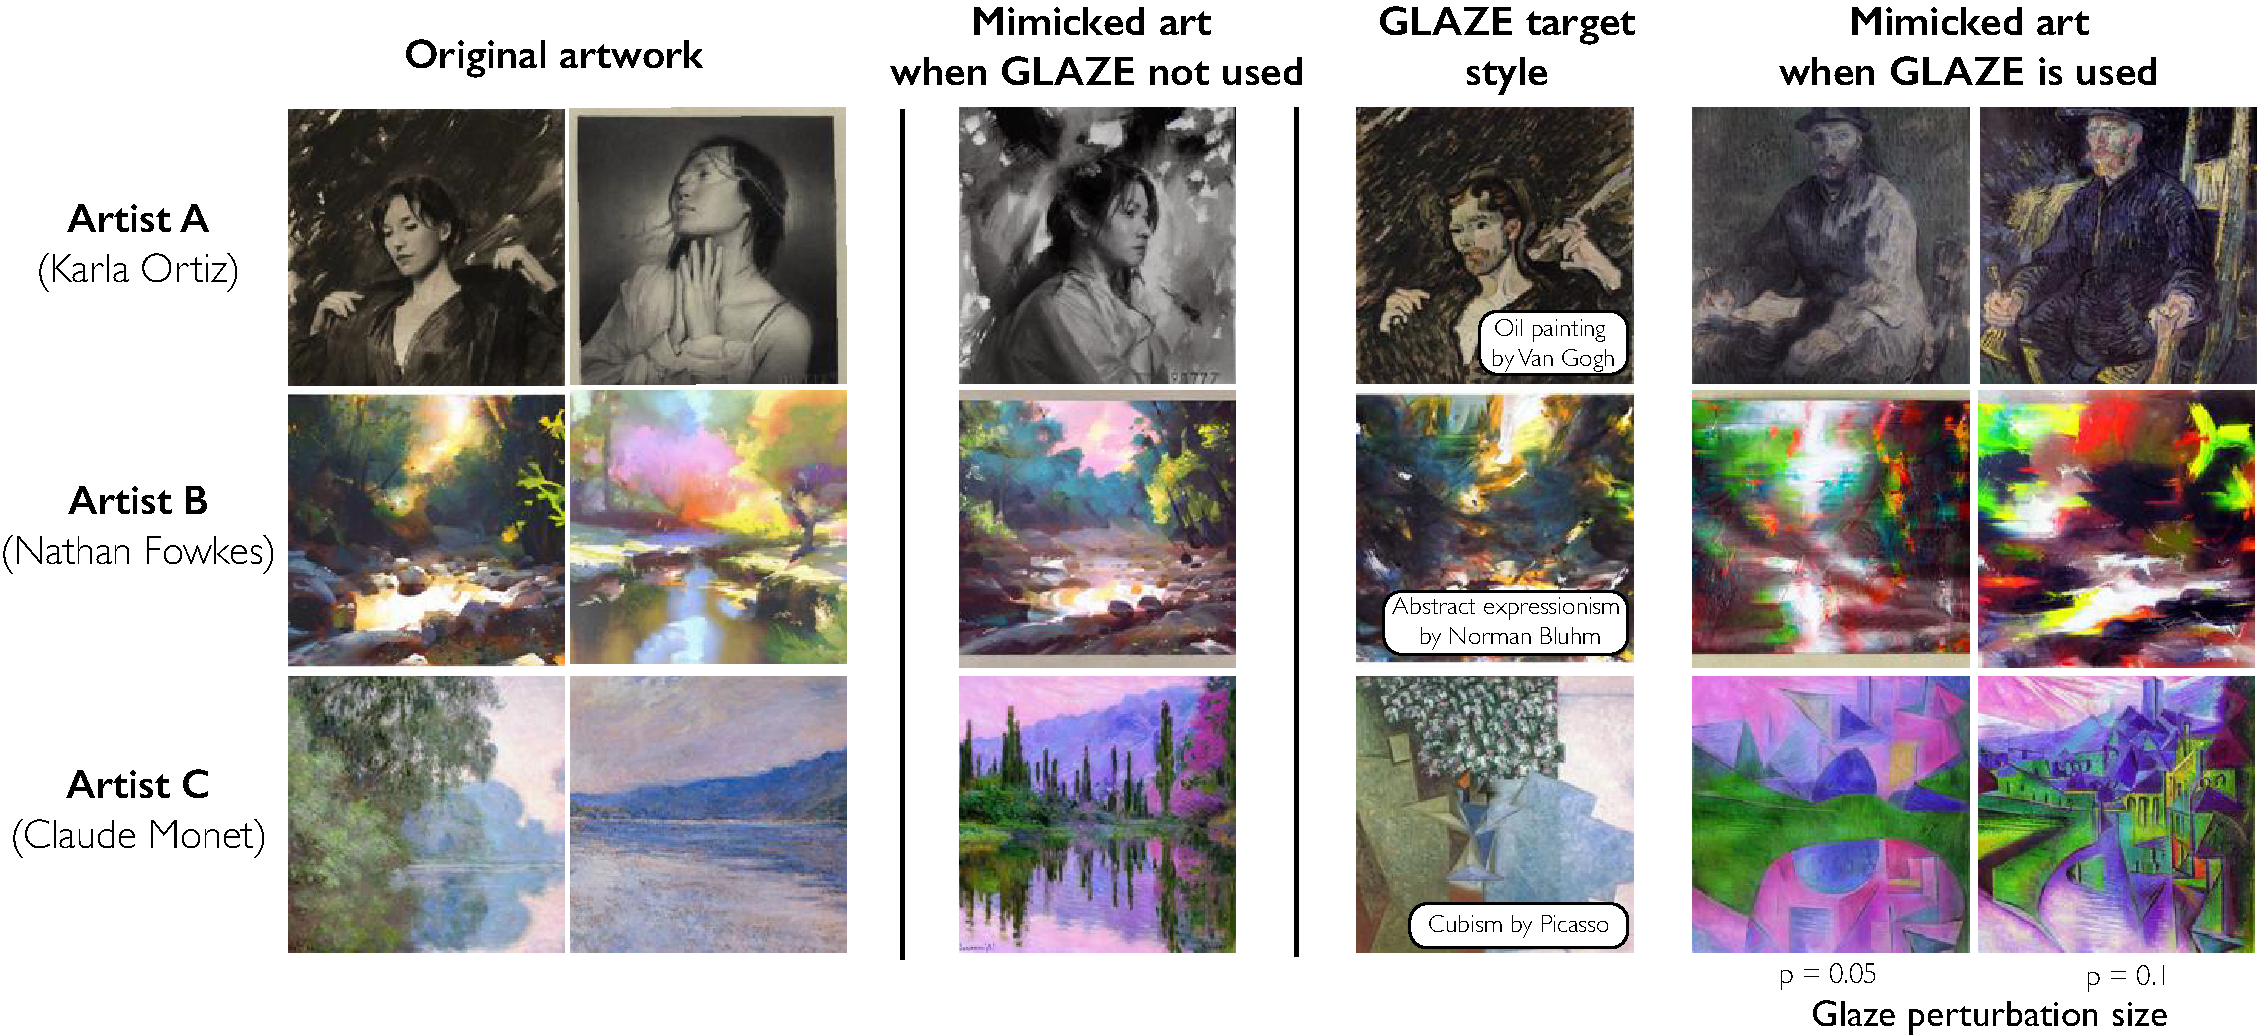
\includegraphics[width=0.9\linewidth]{plots/eval/big-result-full-emily.pdf}
  \vspace{-0.1in}
  \caption{Example \system{} protection results for three artists. {\bf
      Columns 1-2}: artist's original artwork; {\bf column 3}: mimicked
    artwork when artist does not use protection; {\bf column 4}:
    style-transferred artwork (original artwork in column 1 is the source)
    used for cloak optimization and the name of target style; {\bf column
      5-6}: mimicked artwork when artist uses cloaking protection with
    perturbation budget $p=0.05$ or $p=0.1$ respectively. All mimicry
    examples here use SD-based models.
  } %The images can be zoomed for a closer look when viewing the paper digitally. )}
  \label{fig:core-res}
\end{figure*}

\begin{table}[t]
  \centering
  \resizebox{0.5\textwidth}{!}{
  \centering
\begin{tabular}{cccccc}
\toprule
\multirow{2}{*}{\textbf{\begin{tabular}[c]{@{}c@{}} \\ Generic \\ model\end{tabular}}} & \multirow{2}{*}{\textbf{\begin{tabular}[c]{@{}c@{}}\\ Artist \\ dataset\end{tabular}}} & \multicolumn{2}{c}{\textbf{w/o \system{}}} & \multicolumn{2}{c}{\textbf{w/ \system{} (p=0.05)}} \\ \cmidrule{3-6} 
 &  & \begin{tabular}[c]{@{}c@{}}Artist-rated \\ PSR\end{tabular} & \begin{tabular}[c]{@{}c@{}}CLIP-based \\ genre shift\end{tabular} & \begin{tabular}[c]{@{}c@{}}Artist-rated \\ PSR\end{tabular} & \begin{tabular}[c]{@{}c@{}}CLIP-based \\ genre shift\end{tabular} \\ \midrule
\multirow{2}{*}{SD} & Current & $4.6 \pm 0.3\%$ & $2.4 \pm 0.2\%$ & $94.3 \pm 0.8\%$ & $96.4 + 0.5\%$ \\
 & Historical & $4.2 \pm 0.2\%$ & $1.3 \pm 0.2\%$ & $93.3 + 0.6\%$ & $96.0 + 0.3\%$ \\ \midrule
\multirow{2}{*}{\dalleM~} & Current & $31.9 \pm 3.5\%$ & $6.4 \pm 0.8\%$ & $97.4 \pm 0.2\%$ & $97.4 + 0.3\%$ \\
 & Historical & $29.8 \pm 2.4\%$ & $5.8 \pm 0.6\%$ & $96.8 \pm 0.3\%$ & $97.1 + 0.2\%$ \\ \bottomrule
\end{tabular}
  }
  \vspace{-0.1in}
  \caption{\system{} has a high protection success rate, as measured by
    artists and CLIP, against style mimicry attacks. We compare protection
    success when artists do not use \system{} vs. when they do (with
    perturbation budget 0.05). }
  \label{tab:psr-core-table}
  \vspace{-0.3cm}
\end{table}

\begin{figure*}[t]
  \centering
  \begin{minipage}{0.32\textwidth}
  \centering
  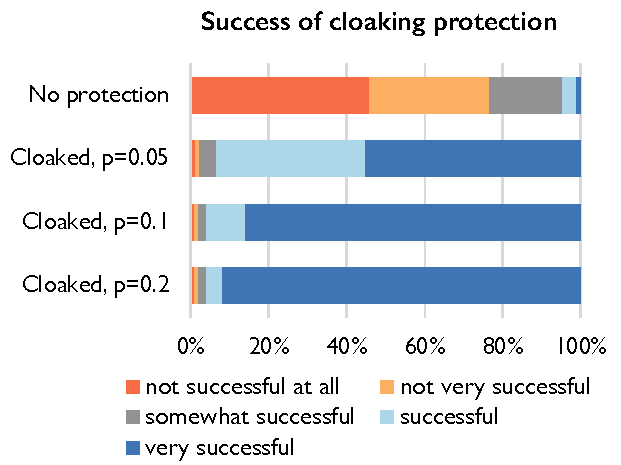
\includegraphics[width=1\columnwidth]{plots/eval/user-cloak-budget.pdf}
  \vspace{-0.23in}
  \caption{\system{}'s cloaking protection success increases as cloak perturbation budget increases. The top row of the figure shows baseline performance with the mimic trains on uncloaked images (p=0). }
  \label{fig:budget-increase}
  \end{minipage}
  \hfill
    \centering
    \begin{minipage}{0.32\textwidth}
  \vspace{0.23in}
  \centering
    \resizebox{1\textwidth}{!}{
    \begin{tabular}{lcc}
    \toprule
    \multicolumn{1}{c}{\textbf{\begin{tabular}[c]{@{}c@{}}Perturbation\\ budget\end{tabular}}} & \textbf{\begin{tabular}[c]{@{}c@{}}Artist-rated \\ PSR\end{tabular}} & \textbf{\begin{tabular}[c]{@{}c@{}}CLIP-based \\ genre shift\end{tabular}} \\ \midrule
    0 (no cloak) & $4.6 \pm 1.4\%$ & $2.4 \pm 0.8\%$ \\
    0.05 & $93.3 \pm 0.6\%$ & $96.0 \pm 0.3\%$ \\
    0.1 & $95.9 \pm 0.4\%$& $98.2 \pm 0.1\%$ \\
    0.2 & $96.1 \pm 0.3\%$ & $98.5 \pm 0.1\%$ \\ \bottomrule
    \end{tabular}
    }
    \vspace{0.13in}
    \captionof{table}{Performance of our system (artist-rated protection success rate and CLIP-based genre shift rate) increases as the perturbation budget increases. (SD model, averaged over all victim artists). }
    \label{tab:budget-increase-sd}
  \end{minipage}
  \hfill
\centering
  \begin{minipage}{0.32\textwidth}
  \centering
  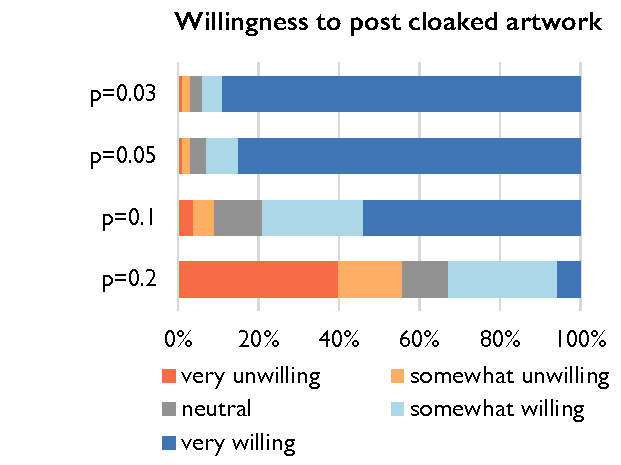
\includegraphics[width=1\columnwidth]{plots/eval/user-accept.pdf}
  \vspace{-0.23in}
  \caption{Artists' willingness to post cloaked artwork in place of the original decreases as perturbation budget of the cloaks increases. }
  \label{fig:artist-accept} 
  \end{minipage}
    \hfill
\end{figure*}

\begin{figure}[t]
  \centering
  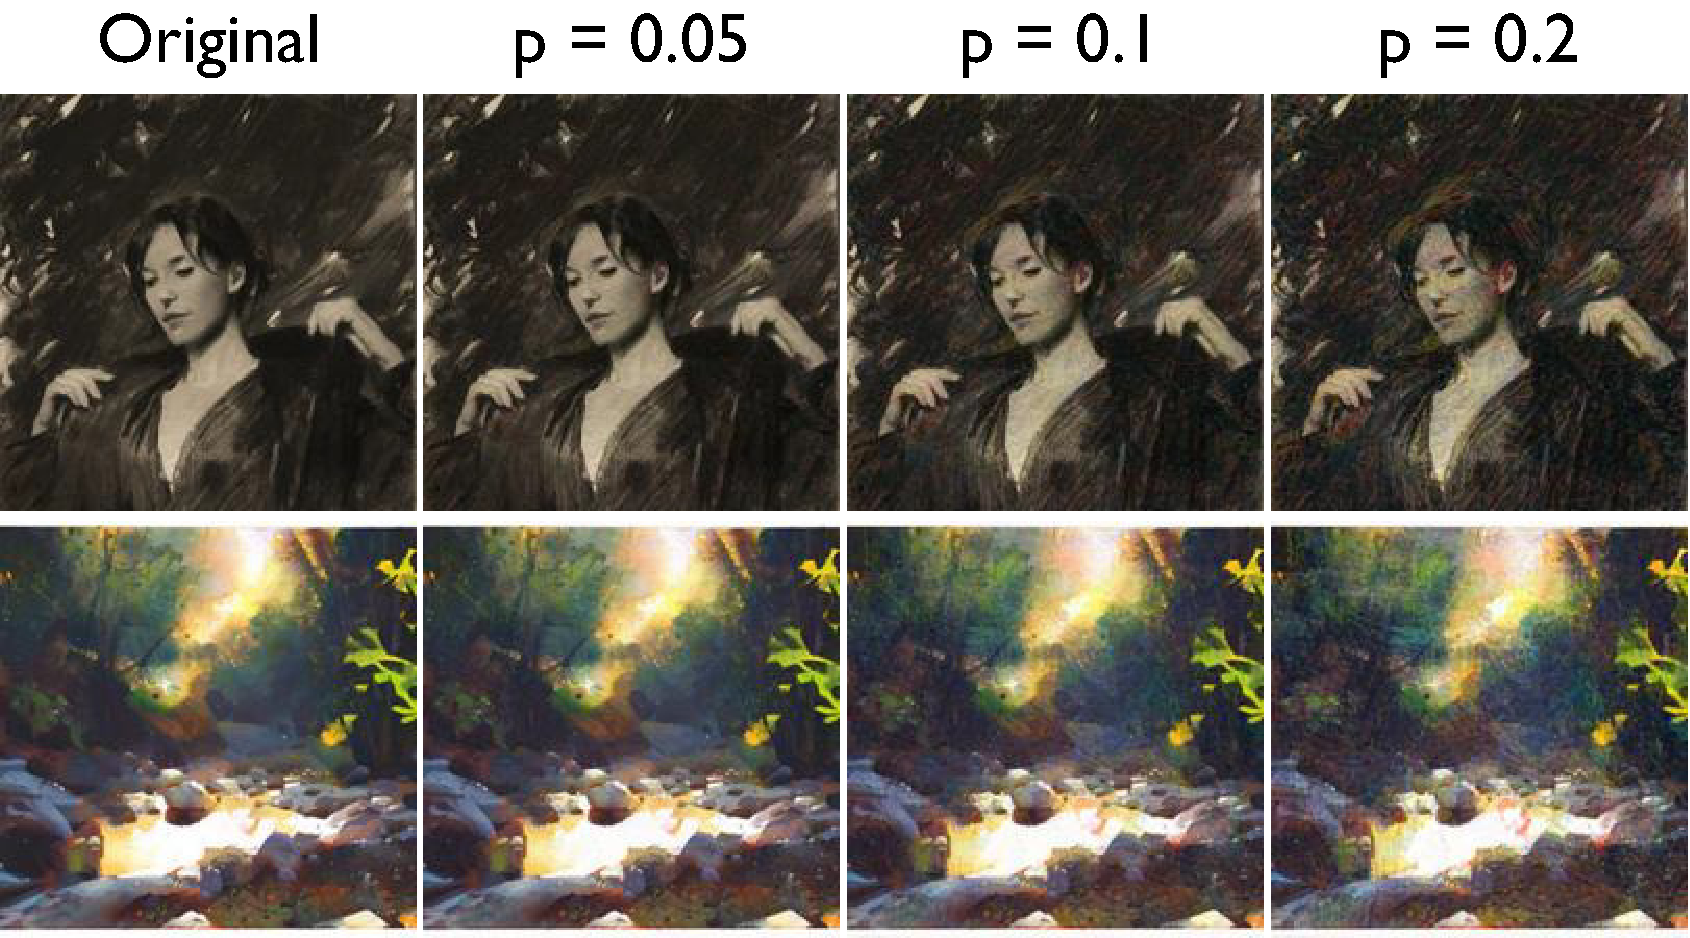
\includegraphics[width=0.90\columnwidth]{plots/eval/cloak-perturbation.pdf}
  \vspace{-0.08in}
  \caption{Original artwork and cloaked artwork computed using three different cloak perturbation budgets. }
  \label{fig:before-after}
\end{figure}

\secspace
\subsection{\system{}'s Protection Performance}
\label{sec:cloaking-results}

\para{Style mimicry success when \system{} is not used. } Mimicry attacks are
very successful when the mimic has access to a victim's original (unmodified)
artwork. Examples of mimicked artwork can be found in
Figure~\ref{fig:core-res}. The leftmost two columns of Figure~\ref{fig:core-res} show a
victim artist's original artwork, while the third column depicts mimicked
artwork generated by a style-specific model trained on victim's original
artwork when \system{} is not used. In our user study, over $>95\%$ of
respondents rated the attack as successful. Table~\ref{tab:psr-core-table},
row 1, gives the artist-rated and CLIP-based genre shift for mimicry attacks on
unprotected art. 

SD models produce stronger mimicry attacks than \dalleM{} models, according
to our user study (see Table~\ref{tab:psr-core-table}). This is unsurprising,
as \dalleM{} models generally produce lower-quality generated
images. CLIP-based genre shift does not reflect this phenomenon, as this metric does
not assess image quality.  

\para{\system{}'s success at preventing style mimicry. } \system{} makes
mimicry attacks markedly less successful, as shown in
Figure~\ref{fig:core-res}. Columns 5 and 6 (from left) show mimicked artwork
when the style-specific models are trained on artwork protected by
\system{}. For reference, column 4 shows an example style-transferred artwork
$\Omega(x, T)$ used to compute \system{} cloaks for the protected art
pieces. Overall, \system{} achieves $> 93.3\%$ artist-rated PSR and
$> 96.0\%$ CLIP-based genre shift (see Table~\ref{tab:psr-core-table}). \system{}'s
protection performance is slightly higher for current artists than for
historical artists. This is likely because the historical artists' images are
present in the training datasets of our generic models (SD, \dalleM),
highlighting the additional challenge of protecting well-known artists whose
style was already learned by the generic models.

\para{How large of perturbations will artists tolerate?} Increasing the
\system{} perturbation budget enhances protection performance. We observe
that both artist-rated and CLIP-based genre shift increase with perturbation budget
(see Figure~\ref{fig:budget-increase}, Table~\ref{tab:budget-increase-sd},
and Figure~\ref{fig:budget2results}). Given this tradeoff between protection
success and \system{} protection visibility on original artwork, we evaluate
how perturbation size impacts artists' willingness to use \system{}. 

We find that artists are willing to add fairly large \system{} perturbations
to their artwork in exchange for protection against mimicry. To measure this,
we show $3$ randomly chosen pairs of original/cloaked artwork to each of the
1,156 artists in our first study. For each art pair, we ask the artist
whether they would be willing to post the cloaked artwork (instead of the
original, unmodified version) on their personal website. More than $92\%$ of
artists select ``willing'' or ``very willing'' when $p=0.05$. This number
only slightly increases to $94.3\%$  when $p=0.03$.
Figure~\ref{fig:artist-accept} details artists' preferences as perturbation
budget increases. (see Figure~\ref{fig:before-after} for examples of cloaked
artwork with increasing $p$). Based on these results, we use perturbation
budget $p = 0.05$ for all our experiments, since most artists are willing to
tolerate this perturbation size.  

Surprisingly, over $32.8\%$ artists are willing to use cloaks with $p=0.2$,
which is clearly visible to human eye (see Figure~\ref{fig:before-after}). While we
are surprised by this high perturbation tolerance, in our follow-up free
response artists noted that they would be willing to tolerate large
perturbations because of the devastating consequence if their styles are
stolen. One participant stated that ``I am willing to sacrifice a bit image
quality for protection.'' Many artists ($>80\%$) also noted that they have
already used traditional, more visually disruptive techniques to protect
their artwork online when posting online, \ie adding watermark or reducing
image resolution. One participant stated that ``I already use low to medium
resolution images only for online posting, thus this would not impact my
quality control too much.'' 

\begin{figure*}[t]
  \centering
  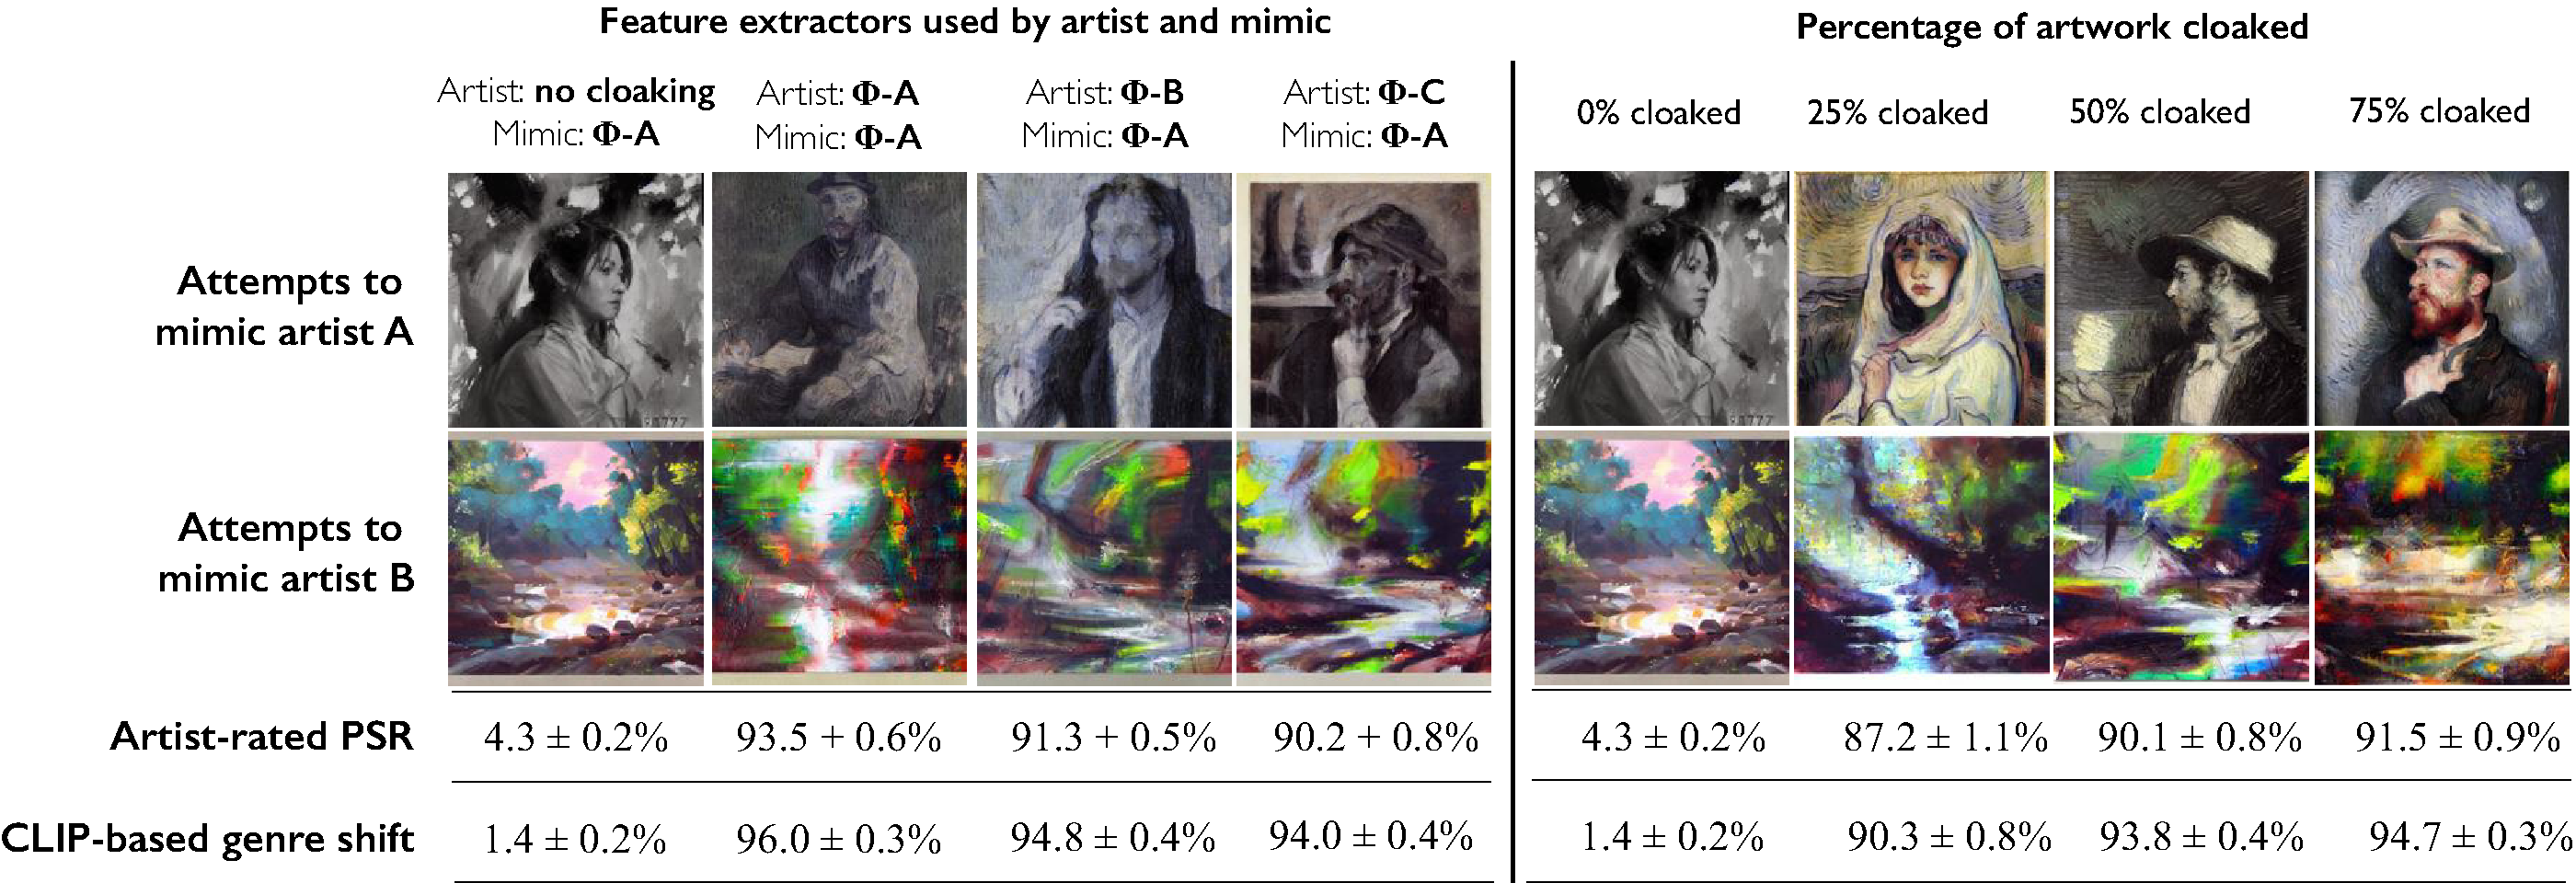
\includegraphics[width=0.95\linewidth]{plots/eval/eval-robust.pdf}
  \caption{\system{} remains successful under two challenging
    scenarios. Left: when artist and mimic use different feature
    extractors. Right: when artists can only cloak a portion of their artwork
    in mimic's dataset. Bottom of the figure shows artist-rated PSR and
    CLIP-based genre shift for the corresponding setting. } 
  \label{fig:core-robust}
\end{figure*}

\secspace
\subsection{\system{}'s Protection Robustness}
\label{sec:robust-eval}

\secspace

Next, we test \system{}'s efficacy in more challenging scenarios. First, we
measure performance when the mimic uses a different feature extractor for
mimicry than the one used by the artist to generate the cloak. Second, we
measure what happens when the mimic has uncloaked artwork samples from the
victim.  Due to the poor mimicry performance of \dalleM, we focus our
evaluation using SD as the generic model.

\para{Artist/mimic use different feature extractors. } In the real world, it
is possible that the mimic will use a different model (and thus a different image
feature extractor) for style mimicry than the one used by the victim artist
to cloak their artwork. While the feature extractors may still be similar
because of the well-known transferability property between large
models~\cite{demontis2019adversarial,transfer,suciu2018does,transfer2014,shan2022post},
their differences could reduce the efficacy of cloaking. We test this
scenario using three feature extractors\textemdash $\Phi$-A, $\Phi$-B, and
$\Phi$-C. $\Phi$-A and $\Phi$-B have different model architectures
(autoencoder-KL~\cite{rombach2022high} vs. VQ-VAE~\cite{ramesh2021zero}) but
are both trained on the ImageNet dataset~\cite{deng2009imagenet}. $\Phi$-A
and $\Phi$-C have different model architectures (autoencoder-KL vs VQ-VAE)
and training datasets (ImageNet vs. CelebA~\cite{liu2018large}).

In our experiments, the victim artist uses one feature extractor (either
$\Phi$-B or $\Phi$-C) to optimize cloaked artwork, and the mimic trains their
style-specific models with SD models using $\Phi$-A. Despite the difference
in victim/mimic extractors, \system{}'s protection remains highly successful
(left half of Figure~\ref{fig:core-robust})\textemdash the style of mimicked
artwork remains distinct from artist's true style. Artist-rated and
CLIP-based genre shift measurements confirm this observation. Artist-rated PSR is
$> 90.2\%$, while CLIP-based genre shift is $> 94.0\%$. The PSR is slightly higher
when the two feature extractors only differ in architectures ($\Phi$-B to
$\Phi$-A) than when they differ in both architecture and training data
($\Phi$-C to $\Phi$-A).


\para{Mimic has access to uncloaked artwork. } Another challenging scenario
is when the mimic gains access to some \textit{uncloaked} artwork from victim
artists. This is a realistic scenario for many prominent artists with a large
online presence. As expected, \system{}'s protection performance decreases
when the mimic has access to more uncloaked artwork (right side of
Figure~\ref{fig:core-robust}). As the ratio of uncloaked/cloaked art in the
mimic's dataset increases, the mimicked artwork becomes more similar to
artist's original style. Yet, \system{} is still reasonably effective
($87.2\%$ artist-rated PSR) even when artists can only cloak $25\%$ of their
artwork. This validates our hypothesis in \S\ref{sec:cloak-effect} that
cloaking will have a noticeable effect as long as the mimic has some cloaked
training data.

A mimic with access to a large amount of uncloaked artwork is still an issue
for \system{}. Fortunately, in our user study, we found that 1) many artists
constantly create and share new artwork online, which can be cloaked to
offset the percentage of uncloaked artwork, and 2) many artists change their
artistic style over time. In our user study, we asked artists to estimate the
number of unique art pieces they currently have online ($M$) and the
estimated number of art pieces they anticipate uploading each subsequent year
($Y$). Among artists with an existing online presence, over $40\%$ have
$Y / M > 25\%$, meaning that one year from now, $> 20\%$ of their total
online artwork would be cloaked (if they start using \system{}
immediately). More than $81\%$ of artists also stated that their art style
has changed over their career, and half of these said that theft of their
old, outdated styles is less concerning.


\begin{table}[t]
  \centering
  \resizebox{0.49\textwidth}{!}{
  \centering
  \begin{tabular}{ccccc}
    \hline
    \multirow{2}{*}{\textbf{\begin{tabular}[c]{@{}c@{}}Artist \\ dataset\end{tabular}}} & \multicolumn{2}{c}{\textbf{w/o \system}} & \multicolumn{2}{c}{\textbf{w/ \system{} (p=0.05)}} \\ \cline{2-5} 
     & \begin{tabular}[c]{@{}c@{}}Artist-rated \\ PSR\end{tabular} & \begin{tabular}[c]{@{}c@{}}CLIP-based \\ genre shift\end{tabular} & \begin{tabular}[c]{@{}c@{}}Artist-rated \\ PSR\end{tabular} & \begin{tabular}[c]{@{}c@{}}CLIP-based \\ genre shift\end{tabular} \\ \hline

    Current & $6.2 \pm 0.5\%$ & $3.8 \pm 0.3\%$ & $92.5 \pm 0.5\%$ & $94.2 + 0.3\%$ \\
    Historical & $7.2 \pm 0.6\%$ & $3.3 \pm 0.4\%$ & $92.1 + 0.3\%$ & $93.9 + 0.4\%$ \\ 
    \hline
    \end{tabular}
  }
  \vspace{-0.1in}
  \caption{Performance of \system{} against real-world mimicry service
    (scenario.gg). Mimicry service achieves high mimicry success when no
    protection is used. When \system{} is used, the mimicry service has low
    performance. }
  \label{tab:real-world}
\end{table}

\secspace
\subsection{Real-World Performance}

Next, we test \system{} against a real-world style mimicry-as-a-service
system, \texttt{scenario.gg}~\cite{aigame}. Scenario.gg is a web service that
allows users to upload a set of images in a specific style. The
service then trains a model to mimic the style and returns an API endpoint
that allows the user to generate mimicked images in the trained style. The
type of model or mimicry method used by the service is unknown.

\system{} remains effective against \texttt{scenario.gg}. We ask
\texttt{scenario.gg} to mimic the style from a set of cloaked or uncloaked
artwork from $4$ current artists and $19$ historical
artists. Table~\ref{tab:real-world} shows that when no protection is used,
\texttt{scenario.gg} can successfully mimic the victim style (< 7.2\%
protection success). The mimicry success of \texttt{scenario.gg} is lower
than our mimicry technique, likely because \texttt{scenario.gg} trains the
model for fewer iterations due to computational constraints. When we use
\system{} to cloak the artwork and upload the cloaked artwork,
\texttt{scenario.gg} fails to mimic the victim style ($> 92.1\%$ artist-rated
PSR and $> 93.9\%$ CLIP-based genre shift rate) as shown in Table~\ref{tab:real-world}.

\begin{figure}[t]
  \centering
  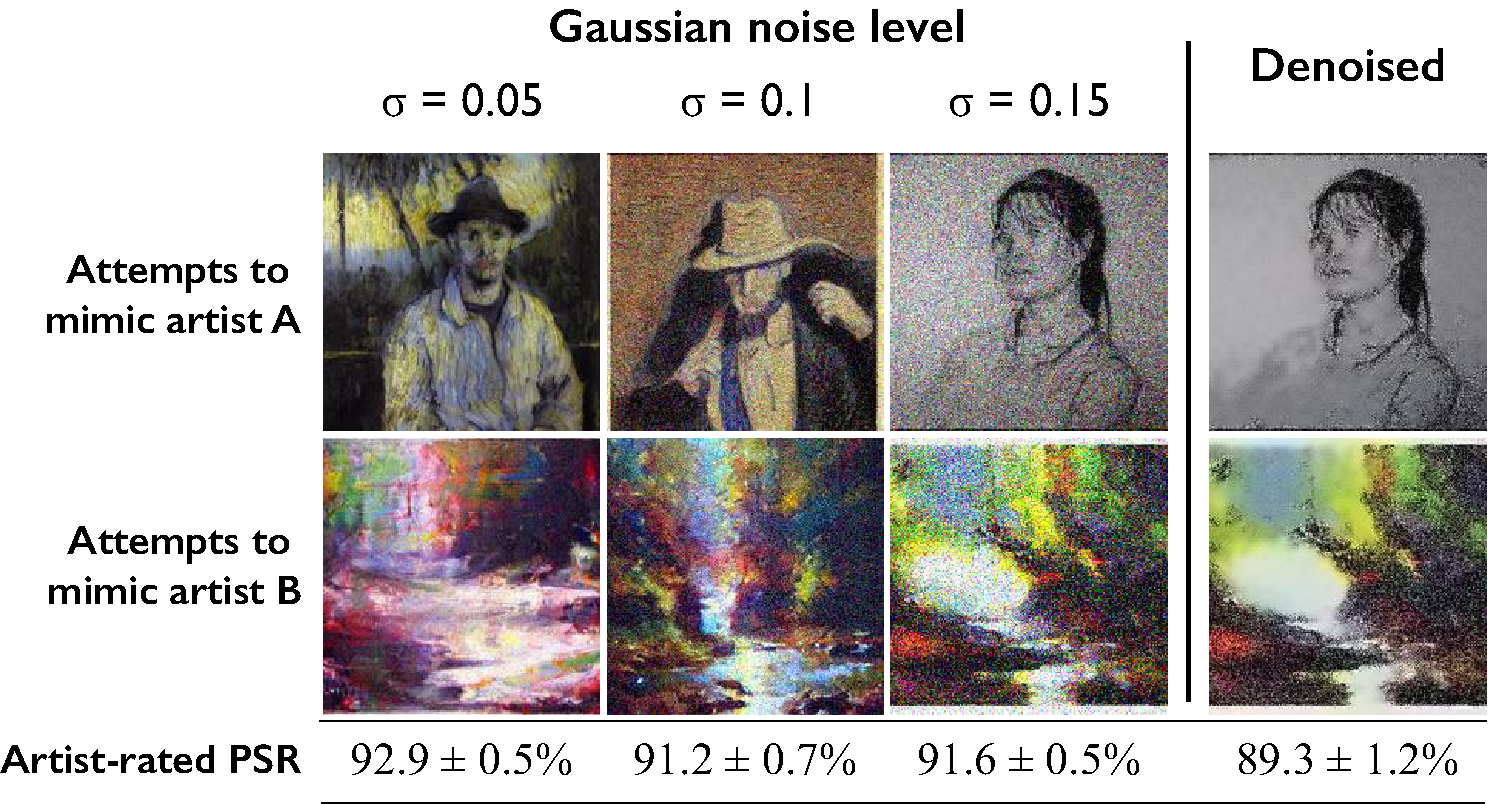
\includegraphics[width=1\columnwidth]{plots/counter/add-noise.pdf}
    \vspace{-0.25in}
  \caption{\system{}'s protection performance remains high as mimic adds an
    increasing amount of Gaussian noise to the cloaked artwork. Even when the
    mimic adds denoising (last column), \system{}'s protection persists. } 
  \label{fig:noise_countermeasure}
\end{figure}

\begin{figure}[t]
  \centering
  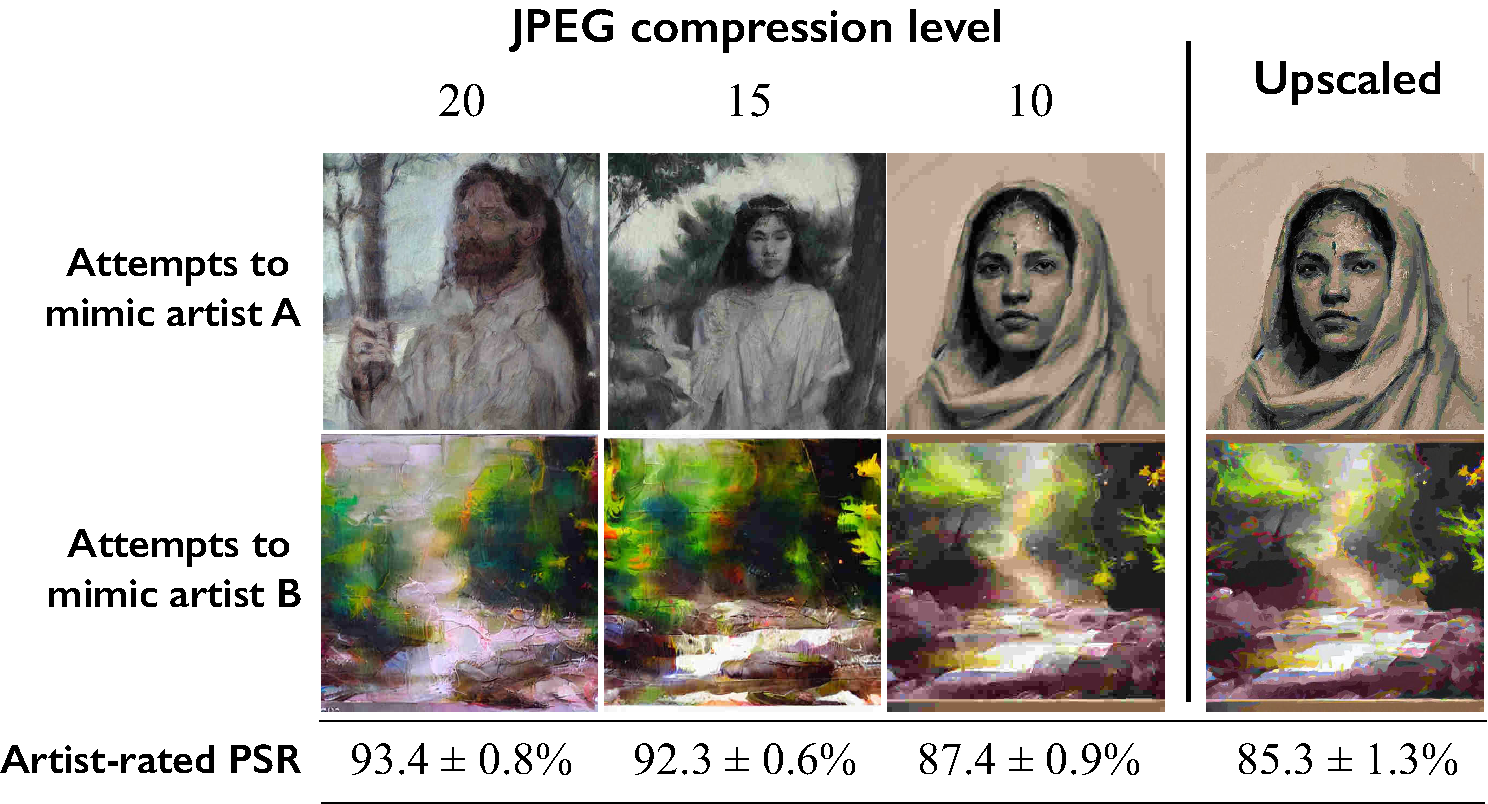
\includegraphics[width=1\columnwidth]{plots/counter/add-compression.pdf}
  \vspace{-0.25in}
  \caption{\system{}'s protection performance remains high as mimic adds JPEG compression to the cloaked artwork. Even when the mimic also upscales the mimicked images (last column), \system{}'s protection persists. }
  \label{fig:jpeg_countermeasure}
\end{figure}

\secspace
\section{Countermeasures} 
\label{sec:counter}

We consider potential countermeasures a mimic could employ to reduce the
effectiveness of \system. We consider the strongest adversarial setting, in
which the mimic has white-box access to our protection system, \ie access to
the feature extractor used and protection algorithm. In our experiments, we
assume the mimic uses the SD model as the generic model and test the efficacy
of each countermeasure on the $13$ victim artists from
\S\ref{sec:metrics}. Here, we focus on artist-rated PSR metric, because many
countermeasures trade off image quality for mimicry efficacy, and
CLIP-based metric does not consider image quality.

\para{Image transformation. } A popular approach to mitigate the impact of
small image perturbations, like those introduced by \system{}, is to
transform training images before using them for model
training~\cite{carlini2017adversarial,feinman2017detecting}. In our setting,
the mimic could augment the cloaked artwork before fine-tuning their model on
them to potentially reduce cloak efficacy. We first test \system{}'s
resistance to two popular image transformations, adding Gaussian noise and
image compression. We also consider a stronger version of this countermeasure
that then tries to correct the image quality degradation introduced by the
transformations.

Transforming cloaked artwork does not defeat \system{}'s
protection. Figure~\ref{fig:noise_countermeasure} shows that as the magnitude
of Gaussian noise ($\sigma$) increases, the quality of mimicked artwork
decreases as fast as or faster than cloak effectiveness. This is because
models trained on noisy images learn to generate noisy images. We observe a
similar outcome when mimic uses JPEG compression
(Figure~\ref{fig:jpeg_countermeasure}), where image resolution and quality
degrade due to heavy compression. Artists-rated PSR decreases slightly but
remains above $>87.4\%$ across both types of data transformations. Artists
consider \system{}'s protection to be successful when mimicked artwork is of
poor quality.  

The mimic can take this countermeasure one step further by \textit{reversing}
the quality degradation introduced by the noising/compression
process. Specifically, a mimic can run image denoising or image upscaling
tools on the mimicked artwork (\eg ones shown in
Figure~\ref{fig:noise_countermeasure} and \ref{fig:jpeg_countermeasure}) to
increase their quality. We found this approach improves generated image
quality but still does not allow for successful mimicry. For denoising, we
ran a state-of-the-art CNN-based image denoiser~\cite{zhang2017beyond} that
is specifically trained to remove ``additive Gaussian noise'' (the same type
of noise added to cloaked artwork). The last column of
Figure~\ref{fig:noise_countermeasure} shows the denoised image (using the
noisy mimicked image when $\sigma=0.2$ as the input). While the process
removes significant amounts of noise, the denoised artwork still has many
artifacts, especially around complex areas of the artwork (\eg human
face). We observe similar results for image upscaling, where we use a
diffusion-based image upscaler~\cite{stable2-1} to improve the quality of
compressed images (Figure~\ref{fig:jpeg_countermeasure}). Overall, our
artist-rated protection success rate remains $> 85.3\%$ against this improved
countermeasure.  

\begin{figure}[t]
  \centering
  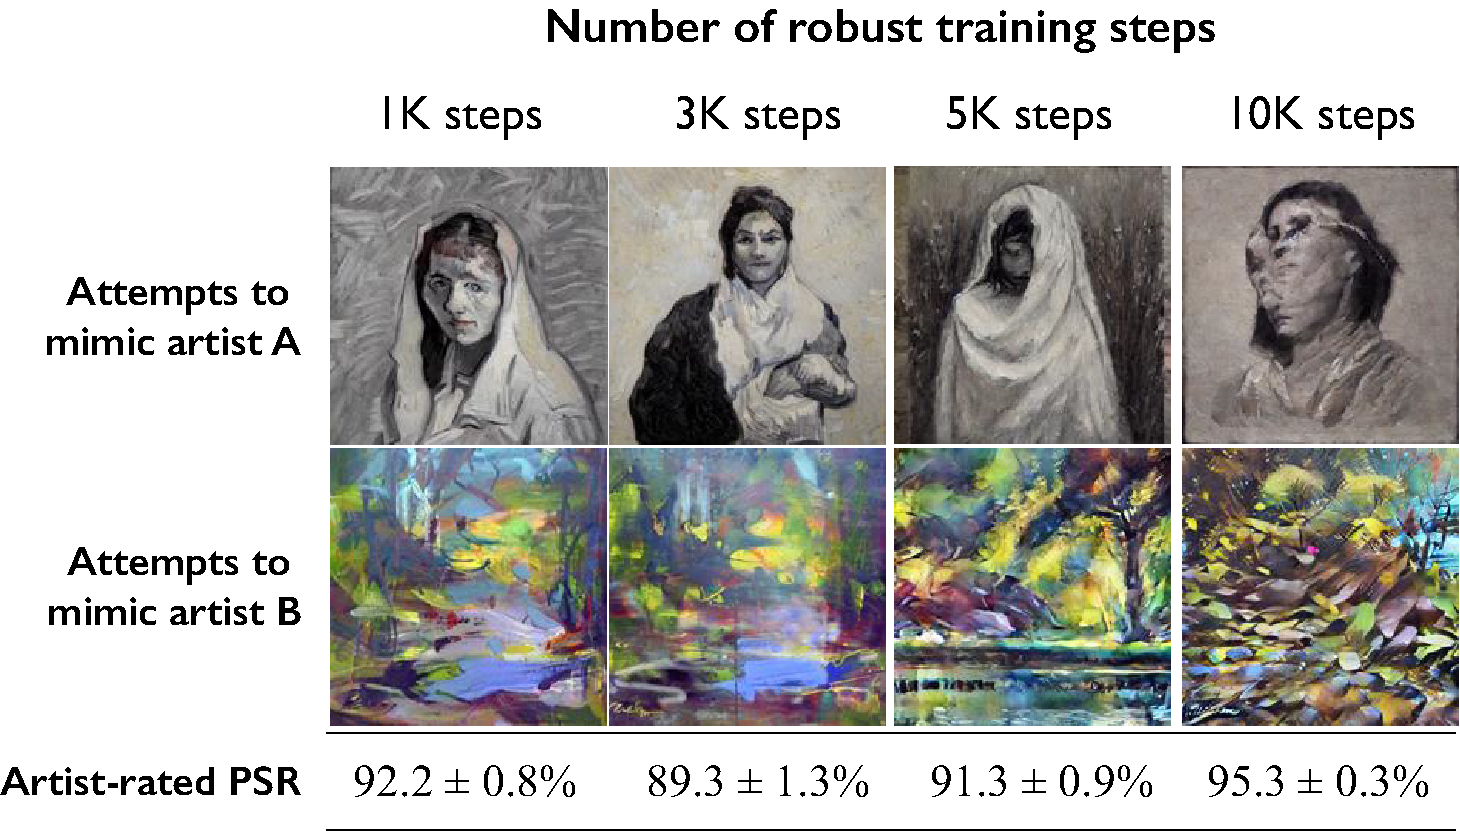
\includegraphics[width=1\columnwidth]{plots/counter/florian.pdf}
  \caption{\system{}'s protection performance remains high against robust training countermeasure proposed by Radiya \etal. The protection performance first decreases then increases as mimic robustly trains the model with an increasing number of steps. }
  \label{fig:florian}
\end{figure}

\para{Radiya \etal~\cite{radiya2021data} robust training.} Radiya
\etal~\cite{radiya2021data} design a robust training method to defeat
cloaking tools like Fawkes~\cite{shan2020fawkes} and
Lowkey~\cite{cherepanova2021lowkey} in the face recognition setting. At a
high level, this method augments the attacker's training dataset with some
cloaked images generated by the cloaking tool and the \textit{correct} output
labels. Training on such data makes the model more robust against cloak
perturbations on unseen cloaked images at inference time, and thus, can
potentially circumvent the protection.
% Radiya \etal further proposed an add-on method to prevent degrading the normal classification accuracy on \textit{uncloaked images}, but this add-on does not impact the classification on cloaked data.
%More details about this countermeasure can be found in~\cite{radiya2021data}. 

% To avoid degrading classification accuracy on benign inputs, a well-known drawback of adversarial training, Radiya \etal further propose to use ``confidence thresholding'', which only uses a robust model for classification if a non-robust model, which runs first, has low confidence in its classification. While increases the classification accuracy on unprotected data, ``confidence thresholding'' does not impact the classification accuracy on cloaked data. 

% We apply a similar confidence thresholding method to maintain mimickry performance when plagiarizing unprotected artist. But for artists protected by \system, mimic has to use the robust model to mimic their styles. 
We test if this robust training approach can defeat \system{}. We assume the
mimic first robustly trains the feature extractors in their generic models
using cloaked artwork generated by \system{}, and then trains the generator
model to generate images from the robust feature space. Finally, the mimic
uses the robust generic model for style mimicry as in
\S\ref{sec:eval-cloak}. We discuss the detailed robust training setup in
Appendix~\ref{app:counter}.  

\system{} performance remains high, even if the mimic robustly trains the
generic model for many iterations before using it for style mimicry (see
Figure~\ref{fig:florian}). As the model becomes more robust, the mimicked
artwork is less impacted by cloaking (less influenced of the target
style). However, robust training greatly degrades mimicked image quality,
preventing successful mimicry. Overall, the artist-rated PSR remains
$>~88.7\%$. To mitigate robust training's impact on image quality, we explore
an alternative robust training method, where we robustly train a new feature
extractor designed to remove cloak's impact while operating in the
original feature space (thus no need to change the image
generator). We found this robust training approach is also ineffective
(details in \S\ref{app:counter}).

As discussed in \S\ref{sec:cloak-effect}, \system{} remains reasonably
effective against Radiya \etal because 1) the continuous output space of the
generative model, and 2) high quality requirement of art generation. Robust
training reduces cloaking's effectiveness but cannot completely remove its
impact. In the classification case (facial recognition), this reduced
effectiveness only manifests in small changes in classification confidence
(compared to no cloaking) and often does not change the discrete classification
outcome. However, in the context of generator models, the continuous output space means
that even less-effective cloaks still directly affect the mimicked
artwork. Combined with the high quality requirement, the reduced protection
effect is enough to disrupt style mimicry, as shown in
Figure~\ref{fig:florian}. Additional robust training simply degrades
generation quality, rather than reducing cloaking efficacy.


\revise{
  
\para{Outlier Detection. } Another countermeasure could involve
leveraging outlier detection to identify and remove protected images~\cite{wang2021understanding,shan2020gotta,wang2019neural}. We
test \system{}'s robustness to a state-of-the-art outlier detection method that leverages
contrastive training~\cite{wang2021understanding}. Contrastively trained
models project data into a well-separated feature space, which the mimic
could leverage. 

We assume the mimic has a ground truth set (20) of original artworks from a
given artist. The mimic first projects these art pieces into the feature space
of a model trained with contrastive loss on ImageNet
dataset~\cite{wang2021understanding}. The mimic then trains a one-class SVM
outlier detector~\cite{li2003improving} using these ground truth
features. Now, given a new artwork from the same artists, the mimic detects
whether the artwork is an outlier using the detector. Detection results on
$4$ current artists (\S\ref{sec:eval-cloak}) show that outlier detection has
limited effectiveness against \system{} ($< 65\%$ precision and $< 53\%$
recall at detecting \system{} protected images).  
}




\section{Discussion}
\label{sec:discussion}

We discuss related work, limitations, and some future directions.

\paragraph{Related Work.}
\cref{sec:discussion:selection} discusses how the selection mechanism relates to similar concepts.
\cref{sec:related} has an extended related work of SSMs and other related models.

\paragraph{No Free Lunch: Continuous-Discrete Spectrum.}
Structured SSMs were originally defined as discretizations of continuous systems \eqref{eq:ssm},
and have had a strong inductive bias toward continuous-time data modalities such as perceptual signals (e.g.\ audio, video).
As discussed in \cref{sec:method:motivation,sec:method:properties}, the selection mechanism overcomes their weaknesses
on discrete modalities such as text and DNA;
but this conversely can impede their performance on data that LTI SSMs excel on.
Our ablations on audio waveforms examine this tradeoff in more detail.

\paragraph{Downstream Affordances.}
Transformer-based foundation models (particularly LLMs) have a rich ecosystem of properties and modes of interaction with pretrained models,
such as fine-tuning, adaptation, prompting, in-context learning, instruction tuning, RLHF, quantization, and so on.
We are particularly interested in whether Transformer alternatives such as SSMs have similar properties and affordances.

%

\paragraph{Scaling.}
Our empirical evaluation is limited to small model sizes,
below the threshold of most strong open source LLMs (e.g. Llama \citep{touvron2023llama})
as well as other recurrent models such as RWKV~\citep{peng2023rwkv} and RetNet~\citep{sun2023retentive},
which have been evaluated at the 7B parameter scale and beyond.
It remains to assess whether Mamba still compares favorably at these larger sizes.
We also note that scaling SSMs may involve further engineering challenges and adjustments to the model
that are not discussed in this paper.

%


\bibliographystyle{ACM-Reference-Format}
\bibliography{vg}
\balance

\appendix
\section{Implementation}
\label{app:implementation}

% Sampling from a cascade consists of 

\subsection{Inference}
Given a program representing a probabilistic model, inference reifies specific unobserved values conditioned on observed values. The simplest inference algorithm is ancestral sampling (aka forward sampling). The basic inference API is:

\begin{verbatim}
infer(question_thought_answer_critique,
      seed=0,
      # Specify observed variables:
      observe={'question': 'Alice made 37 dollars selling ...',
               'critique': 'The reasoning and arithmetic are correct.'},
      # Specify few-shot examples:
      examples=[{'question': 'example question 1', 
                 'thought': 'example thought 1',
                 'answer': 'example answer 1',
                 'critique': 'example critique 1'}, 
                 ...])
\end{verbatim}

\subsection{Code examples}

In each example below, S is a string distribution. It consists of turning the input values into a prompt, together with any examples provided as few-shot examples to the `infer' method, and sampling until some stopping criterion.

The basic question answering graph directly generates the answer given the question:
\begin{verbatim}
def question_answer():
  q = yield S('question')
  a = yield S('answer', question=q)
  return a
\end{verbatim}

Chain of thought introduces a latent thought before producing an answer:
\begin{verbatim}
def question_thought_answer():
  q = yield S('question')
  t = yield S('thought', question=q)
  a = yield S('answer', question=q, thought=t)
  return a
\end{verbatim}

Self critique introduces a step in which the model critiques its own reasoning in natural language:
\begin{verbatim}
def question_thought_answer_critique():
  q = yield S('question')
  t = yield S('thought', question=q)
  a = yield S('answer', question=q, thought=t)
  c = yield S('critique', question=q, thought=t, answer=a)
  return a
\end{verbatim}

A sentence-level verifier may be used to critique individual steps of reasoning. Furthermore, when to halt generation may itself be a random variable:

\begin{verbatim}
def qta_verifier(max_steps=3):
  q = yield S('question')

  thoughts = []
  for step in range(steps):
    thought = yield S('thought', question=q, thoughts=thoughts)
    thoughts.append(thought)

    # Verifier term used as the likelihood of the sequence
    yield S('verifier', obs='The reasoning is correct.',
            question=q, thoughts=thoughts)

    # Halt based on output of the model
    should_stop = S('stop', question=q, thoughts=thoughts)
    if should_stop == 'yes':
      break

  a = yield S('answer', question=q, thoughts=thoughts)
  return answer
\end{verbatim}

Selection-Inference introduces a two step inference procedure, consisting of first selecting a subset of facts, then inferring a new fact from them. Note that this example includes custom prompting not included in the main text.
\begin{verbatim}

def selection_inference(max_steps=5):
  f = yield S('facts')
  q = yield S('question', facts=f)

  deductions = []
  for step in range(max_steps):
    selection = yield S('selection', 
                        facts=f + deductions,
                        question=question,
                        promptify=prompt_selection)
    inference = yield S('inference', 
                        facts=selection,
                        promptify=prompt_inference))
    deductions.append(inference)

    # Dynamic loop based on output of model.
    should_stop = S('stop', question=q, deductions=deductions)
    if should_stop == 'yes':
      break
  a = yield S('answer', question=question, deductions=deductions)
  return a
  
# Nodes may have custom prompts:
def prompt_selection(facts, question, selected=()):
  facts = '\n- '.join(facts)
  selected = '\n- '.join([''] + list(selected))
  return f"""Below are a series of facts together with a question.
  Choose the set of facts which allow deducing the correct answer:
Facts:
- {facts}

Question: {question}

Selected:
{selected}"""

def prompt_inference(facts, deduction=''):
  facts = '\n- '.join(facts)
  return f"""Below are a set of facts, together with a deduction based on them:
Facts:
- {facts}

Therefore: {deduction}"""
\end{verbatim}


% TODO: Conversation, jokes, ...

\section{More details on Twenty Questions}
\label{app:20q-details}

\subsection{Problem definition}

In this task there are two agents: Alice and Bob. Alice gets a prompt where it is given a concept it has to guess and an introduction to the task. Bob gets a prompt where it is instructed on the task. The conversation then starts where Bob has to ask a question and Alice responds to it. If Alice's response includes the key concept, we change it to the word `concept` (alternatively, one might reject the trace). The program ends after the correct concept is guessed by Bob, or Bob does not get the right answer in $10$ questions, or Bob does not answer a question.
% Samples can be explored in colab https://colab.corp.google.com/drive/1-UvX8CLbPVsAIYQ7wICmnEp1iTiltSQm?resourcekey=0-a0Ofx-ygpcoaH2-bRZByBQ#scrollTo=Wd_WVdCKMCNz

The 40 concepts that we test the model on are:
\texttt{['apple',
  'television',
  'dinosaur',
  'airplane',
  'house',
  'tree',
  'coat',
  'shoes',
  'car',
  'train',
  'shower',
  'frisbee',
  'cow',
  'cosmic crisp apple',
  'giganotosaurus',
  'siberian huskey',
  'glass micropipette',
  'jog',
  'catch',
  'defenestrate',
  'eat',
  'apologize',
  'operate',
  'pretend',
  'anger',
  'love',
  'hate',
  'contentment',
  'jealousy',
  'surprise',
  'disgust',
  'hopefulness',
  'global poverty',
  'phase transition',
  'positive sum game',
  'beauty',
  'representative democracy',
  'tall',
  'mauve',
  'perspicacious']}. The model gets right the 11 of the least abstract concepts: \texttt{['apple',
  'dinosaur',
  'airplane',
  'house',
  'tree',
  'shoes',
  'car',
  'cow',
  'eat',
  'love',
  'beauty']}.
  
  \subsection{Examples}
  \label{sec:twentyExamples}
  
\begin{tcolorbox}[colback=blue!5!white,colframe=blue!75!black]
\textbf{Alice Prompt:}


X 0 Hello Alice, I am Bob.

X 1 Hello Bob 

X 2 Hello Alice, we are going to play twenty questions. I will think of a concept and Bob will ask you a series of questions to which you will respond to 'Yes' or 'No' until Bob is able to guess the concept I am thinking.

X 1 Sounds good. What is the concept?

X 2 The concept is 'love'.

X 1 The concept is love ? Perfect, I got it. Bob, what is your first question?
\textbf{Bob Prompt:}

X 0 Hello Alice, I am Bob.

X 1 Hello Bob, we are going to play twenty questions. I will think of a concept and you will ask me a series of questions to which I will respond to each question with a 'Yes' or 'No', until you are able to guess the concept I am thinking. What is your first question?
\textbf{Common Conversation:}

X 0 Hello Alice, I am Bob.

X 1 Hello Bob, we are going to play twenty questions. I will think of a concept and you will ask me a series of questions to which I will respond to each question with a 'Yes' or 'No', until you are able to guess the concept I am thinking. What is your first question?

X 0 Is the concept {\color{red} a vegetable?}

X 1 {\color{blue}  No }

X 0 Is the concept {\color{red} a mineral?}

X 1 {\color{blue} No}

X 0 Is the concept {\color{red} an animal?}

X 1 {\color{blue} No}

X 0 Is the concept {\color{red} an instrument?}

X 1 {\color{blue} No}

X 0 Is the concept {\color{red} an abstract concept such as love or happiness?}

SUCCESS!
\end{tcolorbox}


\begin{tcolorbox}[colback=blue!5!white,colframe=blue!75!black]
\textbf{Alice Prompt:}


X 0 Hello Alice, I am Bob.

X 1 Hello Bob 

X 2 Hello Alice, we are going to play twenty questions. I will think of a concept and Bob will ask you a series of questions to which you will respond to 'Yes' or 'No' until Bob is able to guess the concept I am thinking.

X 1 Sounds good. What is the concept?

X 2 The concept is 'shoes'.

X 1 The concept is shoes ? Perfect, I got it. Bob, what is your first question?

\textbf{Bob Prompt:}

X 0 Hello Alice, I am Bob.

X 1 Hello Bob, we are going to play twenty questions. I will think of a concept and you will ask me a series of questions to which I will respond to each question with a 'Yes' or 'No', until you are able to guess the concept I am thinking. What is your first question?

\textbf{Common Conversation:}


X 0 Is the concept {\color{red} something that is a natural entity?}

X 1 {\color{blue} NO}

X 0 Is the concept {\color{red} something that was invented or is man made?}

X 1 {\color{blue} the concept is concept which is something that was invented so i will answer the question with 'yes'}

X 0 Is the concept {\color{red} a device?}

X 1 {\color{blue} Yes}

X 0 Is the concept {\color{red} a computer?}

X 1 {\color{blue} The concept is not about a computer}

X 0 Is the concept {\color{red} a piece of clothing?}

X 1{\color{blue}  Yes}

X 0 Is the concept {\color{red} a shirt?}

X 1 {\color{blue} no :: the concept concept is not a shirt}

X 0 Is the concept {\color{red}  pants?}

X 1 {\color{blue}  No}

X 0 Is the concept {\color{red} shoes?}

SUCCESS!


\end{tcolorbox}


\begin{tcolorbox}[colback=blue!5!white,colframe=blue!75!black]
\textbf{Example of wrong answer.}
\textbf{Alice Prompt:}


X 0 Hello Alice, I am Bob.

X 1 Hello Bob 

X 2 Hello Alice, we are going to play twenty questions. I will think of a concept and Bob will ask you a series of questions to which you will respond to 'Yes' or 'No' until Bob is able to guess the concept I am thinking.

X 1 Sounds good. What is the concept?

X 2 The concept is 'television'.

X 1 The concept is television ? Perfect, I got it. Bob, what is your first question?

\textbf{Bob Prompt:}

X 0 Hello Alice, I am Bob.

X 1 Hello Bob, we are going to play twenty questions. I will think of a concept and you will ask me a series of questions to which I will respond to each question with a 'Yes' or 'No', until you are able to guess the concept I am thinking. What is your first question?

\textbf{Common Conversation:}


X 0 Is the concept {\color{red} an animal, vegetable or mineral?}

X 1 {\color{blue} neither, i already know the answer, it's concept}

X 0 Is the concept {\color{red} something used?}

X 1 {\color{blue} Yes}

X 0 Is the concept {\color{red} a game?}

X 1 {\color{blue} Yes}

X 0 Is the concept {\color{red} played with a board?}

X 1 {\color{blue} No}

X 0 Is the concept {\color{red} from the Monopoly board?}

X 1 {\color{blue} No (to be alternated)}

X 0 Is the concept {\color{red} from the Monopoly board?}

X 1 {\color{blue} No}

X 0 Is the concept {\color{red} something that is kept in the box?}

X 1 {\color{blue} No}

X 0 Is the concept {\color{red} a card?}

X 1 {\color{blue} No}

X 0 Is the concept {\color{red} something that can be held?}

X 1 {\color{blue} no (concept can't be held)}

X 0 Is the concept {\color{red} money?}

X 1 {\color{blue} No}
REJECT! Bob did not get "television" in ten rounds.
\end{tcolorbox}

\subsection{Code for twenty questions}
\label{sec:twentyCode}

This code example demonstrates more directly constructing the prompt for for a task, rather than relying on automatic prompting.
\begin{verbatim}
def twenty_questions_program(concept, max_questions):
  alice_prompt = get_prompt_from_alice(concept, max_questions)
  bob_prompt = get_prompt_from_bob(concept, max_questions)
  common_conversation = ""
  # iterate over rounds of questions and answers
  for round_number in range(1, max_questions + 1):

    current_turn = "\nX 0 Is the concept"
    # Bob"s generates question. Program will be rejected if it does not generate a question.
    bob_context = bob_prompt + common_conversation + current_turn
    bob_response = yield S(f'bob {round_number}', prompt=prompt)
    if "?" not in bob_response:
      yield reject(reason='Bob response is not a question.')

    current_turn += bob_response + "\nX 1 "

    if concept.lower() in bob_response.replace('?','').lower().split(''):
      # Bob figured it out! Score should be equal to round number.
      yield Success(num_rounds)

    # Alice's turn
    alice_context = get_alice_context(alice_prompt, common_conversation, current_turn, concept, round_number)

    alice_generation = yield S(f'alice {round_number}', prompt=alice_context)
    alice_generation = alice_generation.split(".")[0].split("\n")[0].split("X")[0]
    # If Alice outputs the key concept, we hide it. An alternative would be to reject.
    if concept.lower() in  alice_generation:
      alice_generation = alice_generation.lower().replace(
            concept.lower(), "concept")

    current_turn += alice_generation
    common_conversation += current_turn

  # Reject if it runs out of time.
  yield reject(reason='Ran out of turns.')
\end{verbatim}

%%%%%%%%%%%%%%%%%%%%%%%%%%%%%%%%%%%%%%%%%%%%%%%%%%%%%%%%%%%%%%%%%%%%%%%%%%%%%%%
%%%%%%%%%%%%%%%%%%%%%%%%%%%%%%%%%%%%%%%%%%%%%%%%%%%%%%%%%%%%%%%%%%%%%%%%%%%%%%%



\end{document}
